\documentclass[semifinal]{cpecmu}

%% This is a sample document demonstrating how to use the CPECMU
%% project template. If you are having trouble, see "cpecmu.pdf" for
%% documentation.

\projectNo{P021-2/65}
\acadyear{2022}

\titleTH{เว็ปไซตทยท}
\titleEN{Website for organize and manage tournaments}

\author{นายภูเบศ รุจิเรกานุสรณ์}{Phubet Rujirekanusorn}{620610804}

\cpeadvisor{chinawat}
\cpecommittee{paskorn}
\committee{รศ.ดร.\,นิพนธ์ ธีรอำพน}{Assoc.\,Prof.\,Nipon Theera-Umpon, Ph.D.}

%% Some possible packages to include:
\usepackage[final]{graphicx} % for including graphics

%% Add bookmarks and hyperlinks in the document.
\PassOptionsToPackage{hyphens}{url}
\usepackage[colorlinks=true,allcolors=Blue4,citecolor=red,linktoc=all]{hyperref}
\def\UrlLeft#1\UrlRight{$#1$}

%% Needed just by this example, but maybe not by most reports
\usepackage{afterpage} % for outputting
\usepackage{pdflscape} % for landscape figures and tables. 

%% Some other useful packages. Look these up to find out how to use
%% them.
% \usepackage{natbib}    % for author-year citation styles
% \usepackage{txfonts}
% \usepackage{appendix}  % for appendices on a per-chapter basis
% \usepackage{xtab}      % for tables that go over multiple pages
% \usepackage{subfigure} % for subfigures within a figure
% \usepackage{pstricks,pdftricks} % for access to special PostScript and PDF commands
% \usepackage{nomencl}   % if you have a list of abbreviations

%% if you're having problems with overfull boxes, you may need to increase
%% the tolerance to 9999
% \tolerance=9999

\bibliographystyle{plain}
% \bibliographystyle{IEEEbib}

% \renewcommand{\topfraction}{0.85}
% \renewcommand{\textfraction}{0.1}
% \renewcommand{\floatpagefraction}{0.75}

%% Example for glossary entry
%% Need to use glossary option
%% See glossaries package for complete documentation.
\ifglossary
  \newglossaryentry{lorem ipsum}{
    name=lorem ipsum,
    description={derived from Latin dolorem ipsum, translated as ``pain itself''}
  }
\fi

%% Uncomment this command to preview only specified LaTeX file(s)
%% imported with \include command below.
%% Any other file imported via \include but not specified here will not
%% be previewed.
%% Useful if your report is large, as you might not want to build
%% the entire file when editing a certain part of your report.
% \includeonly{chapters/intro,chapters/background}

\begin{document}
\maketitle
\makesignature

\ifproject
\begin{abstractTH}
% เขียนบทคัดย่อของโครงงานที่นี่

% การเขียนรายงานเป็นส่วนหนึ่งของการทำโครงงานวิศวกรรมคอมพิวเตอร์
% เพื่อทบทวนทฤษฎีที่เกี่ยวข้อง อธิบายขั้นตอนวิธีแก้ปัญหาเชิงวิศวกรรม และวิเคราะห์และสรุปผลการทดลองอุปกรณ์และระบบต่างๆ
% \enskip อย่างไรก็ดี การสร้างรูปเล่มรายงานให้ถูกรูปแบบนั้นเป็นขั้นตอนที่ยุ่งยาก
% แม้ว่าจะมีต้นแบบสำหรับใช้ในโปรแกรม Microsoft Word แล้วก็ตาม
% แต่นักศึกษาส่วนใหญ่ยังคงค้นพบว่าการใช้งานมีความซับซ้อน และเกิดความผิดพลาดในการจัดรูปแบบ กำหนดเลขหัวข้อ และสร้างสารบัญอยู่
% \enskip ภาควิชาวิศวกรรมคอมพิวเตอร์จึงได้จัดทำต้นแบบรูปเล่มรายงานโดยใช้ระบบจัดเตรียมเอกสาร
% \LaTeX{} เพื่อช่วยให้นักศึกษาเขียนรายงานได้อย่างสะดวกและรวดเร็วมากยิ่งขึ้น

โครงงานนี้ได้นําเสนอเว็บไซต์ที่ใช้ในการให้บริการ จัดสร้าง และจัดการทัวร์นาเมนต์ที่ครบจบในที่เดียว 
อีกทั้งยังมีระบบในการเก็บประวัติให้แก่ผู้เล่นให้นําไปใช้เป็นที่สะสมผลงาน และนําไปสานต่อในการเป็นผู้เล่น eSport ในอนาคต โดยเว็บไซต์ฝั่ง Frontend จะถูกพัฒนาด้วย React framework ใช้ภาษา JavaScript 
ฝั่งBackend จะถูกพัฒนาด้วย Nest framework ใช้ภาษา TypeScript ในส่วนของฐานข้อมูลใช้การจัดเก็บข้อมูลแบบSQL ร่วมกับ PostgreSQL ในการจัดการ และใช้Google Firebase Cloud Storage 
ในการจัดเก็บรูปภาพ
\end{abstractTH}

\begin{abstract}


    This project presents a website that can be used to serve, organize and manage tournament all in one website. there is also a system to collect history for player to use as portfolio.And lead to future participation in E-sport Career. 
The website's Forntend site will be developed with React framework using JavaScript. 
On the Backend site will be developed with Nest using TypeScript.
For the database use SQL for storage with PostgreSQL and Google Firebase Cloud Storage to store images.
\end{abstract}

% \iffalse
% \begin{dedication}
% This document is dedicated to all Chiang Mai University students.

% Dedication page is optional.
% \end{dedication}
% \fi % \iffalse

% \begin{acknowledgments}
% Your acknowledgments go here. Make sure it sits inside the
% \texttt{acknowledgment} environment.

% \acksign{2020}{5}{25}
% \end{acknowledgments}%
% \fi % \ifproject

\contentspage

\ifproject
\figurelistpage

\tablelistpage
\fi % \ifproject

% \abbrlist % this page is optional

% \symlist % this page is optional

% \preface % this section is optional


\pagestyle{empty}\cleardoublepage
\normalspacing \setcounter{page}{1} \pagenumbering{arabic} \pagestyle{cpecmu}

\chapter{\ifenglish Introduction\else บทนำ\fi}

\section{\ifenglish Project rationale\else ที่มาของโครงงาน\fi}
เนื่องจากการแข่งขัน E-sport กำลังเติบโตเป็นอย่างมากและเป็นที่นิยมขึ้นเรื่อยๆ ในการจัดการแข่งขันทัวร์นาเมนต์นั้น
ต้องใช้หลายแอพพลิเคชันในการจัดการทั้งใช้ในการจัดการคน การทำตารางแข่ง การเก็บบันทึกผล และการแสดงผลลัพธ์ ซึ่งต้องใช้
แอพพลิเคชันหลายอัน เช่น Excel, Photoshop และ Google Dirve   จึงเป็นที่มาของโครงงานนี้ที่จะนำสิ่งต่างๆที่จำเป็นมาไว้ในเว็ปไซต์นี้เว็ปไซต์เดียว
และ อีกหนึ่งเหตุผลก็คือต้องการยกระดับวงการ E-sport และให้โอกาศแก่ผู้ที่ต้องการเริ่มต้นเข้าสู่วงการที่ไม่ได้มีทุนมากมาย แต่มีใจที่จะมาสายงานนี้  


\section{\ifenglish Objectives\else วัตถุประสงค์ของโครงงาน\fi}
\begin{enumerate}
    \item พัฒนาเว็บแอพพลิเคชันที่ใช้ในการจัดสร้าง และจัดการทัวร์นาเมนต์ ได้ในที่เดียว
    \item ใช้เป็นที่เก็บผลงานของเหล่านักกีฬา E-sport ได้
    \item สามารถนำไปใช้ต่อยอดและใช้จริงได้ในอนาคต
\end{enumerate}

\section{\ifenglish Project scope\else ขอบเขตของโครงงาน\fi}

\subsection{\ifenglish Software scope\else ขอบเขตด้านซอฟต์แวร์\fi}
\begin{enumerate}
    \item การสร้างทัวร์นาเมนต์จะมีแค่แบบเดียวคือ Double-elimination tournament \cite{tournament}
    \item สร้างทัวร์นาเมนต์จากเกมที่มีในระบบได้เท่านั้น 
    \item สามรถจัดเก็บประวัติ และจัดการโปรไฟล์ได้ตามที่มีกำหนดให้เท่านั้น
    \item การกำหนดผลการแข่งขั้นนั้นขึ้นอยู่กับผู้จัดการแข่งขันเป็นผู้จัดการไม่สามรถตรวจสอบเพื่อยืนยันได้
    \item ระบบความปลอดภัยขอเว็ปไซต์ใช้เพียงแค่ Token เท่านั้น
\end{enumerate}

\section{\ifenglish Expected outcomes\else ประโยชน์ที่ได้รับ\fi}
\begin{enumerate}
    \item ช่วยอำนวยความสะดวกให้ผู้ดูแลการแข่งขัน
    \item เป็นที่เก็บผลงานประวัติการแข่งขันของผู้เข้าแข่งขัน
    \item สามารถนำไปใช้ร่วมกับโปรเจค StartUp ของทีมผมเพื่อสร้าง Ecosystem ของวงการ E-sport
\end{enumerate}

\section{\ifenglish Technology and tools\else เทคโนโลยีและเครื่องมือที่ใช้\fi}

\subsection{\ifenglish Software technology\else เทคโนโลยีด้านซอฟต์แวร์\fi}
\begin{enumerate}
    \item React\cite{react} - Open-source Fontend library ของ JavaScript เพื่อใช้สร้างหน้า User Interface
    \item JavaScript\cite{javascript} - ภาษาโปรแกรมมิ่งที่ใช้ในการเขียนหน้าเว็ปไซต์
    \item Nest\cite{nest} - Progressive Framework สำหรับการสร้างแอพพลิเคชันสวน Backend ที่มีประสิทธิภาพ มีความน่าเชื่อถือ และสามารถขยายได้
    \item TypeScript\cite{typescript} - ภาษาโปรแกรมมิ่งที่มีความเคร่งครัดในชนิดของตัวแปลที่พัฒนามาจาก Javascript
    \item PostgreSQL\cite{postgresql} - ระบบการจัดการฐานข้อมูล object-relational โดยสามารถใช้รูปแบบคำสั่งของภาษา SQL
    \item Firebase Cloud Storage\cite{firebase} - Clound Storage สำหรับจัดเก็บข้อมูลเพื่อใช้ในการแสดง content เช่นรูป และ วีดีโอ
    \item Postman\cite{postman} - เครื่องมือที่ใช้ใช้ในการเขียน API Document และใช้ทดสอบการทำงานของ API
    \item Figma\cite{figma} - เครื่องมือที่ใช้ในการออกแบบหน้าเว็ปไซต์
\end{enumerate}

\section{\ifenglish Project plan\else แผนการดำเนินงาน\fi}

\begin{plan}{9}{2022}{3}{2023}
    \planitem{9}{2022}{10}{2022}{ออกแบบUX/UI เลือกเครื่องมือ และเขียนรายงาน}
    \planitem{10}{2022}{11}{2022}{พัฒนาฐานข้อมูล}
    \planitem{11}{2022}{3}{2023}{พัฒนาเว็ปแอพพลิเคชัน}
    \planitem{3}{2023}{3}{2023}{ทดสอบกับกลุ่มผู้ใช้งานเป้าหมาย}
    \planitem{3}{2023}{3}{2023}{สรุปผล และจัดเตรียมนำเสนอ}
\end{plan}
\begin{center}
    **ทำการเปลี่ยนหัวข้อโปรเจคเมื่อวันที่ 24 ก.ย. 2565**
\end{center}

% \section{\ifenglish Roles and responsibilities\else บทบาทและความรับผิดชอบ\fi}
% ออกแบบ พัฒนา ไปทดสอบ

\section{\ifenglish%
Impacts of this project on society, health, safety, legal, and cultural issues
\else%
ผลกระทบด้านสังคม สุขภาพ ความปลอดภัย กฎหมาย และวัฒนธรรม
\fi}

ในการทำโครงงานนี้คาดว่าจะช่วยลดขั้นตอน และความยุ่งยากในการจัดสร้าง และจัดการทัวร์นาเมนต์
มากไปกว่านั้นเว็ปไซต์นี้จะเป็นศูนร่วมของเหล่านักกีฬา E-sport และเหล่าผู้จัดการแข่งขันในอานาคต

\chapter{\ifenglish Background Knowledge and Theory\else ทฤษฎีที่เกี่ยวข้อง\fi}

การทำโครงงาน เริ่มต้นด้วยการศึกษาค้นคว้า ทฤษฎีที่เกี่ยวข้อง หรือ งานวิจัย/โครงงาน ที่เคยมีผู้นำเสนอไว้แล้ว ซึ่งเนื้อหาในบทนี้ก็จะเกี่ยวกับการอธิบายถึงสิ่งที่เกี่ยวข้องกับโครงงาน เพื่อให้ผู้อ่านเข้าใจเนื้อหาในบทถัดๆ ไปได้ง่ายขึ้น

\section{UX Design}
UX Design(User Experience Design) คือ การออกแบบเพื่อให้ผู้ใช้งานมีประสบการณ์ในการใช้งานที่ดีในเว็ปไซต์ หรือแอพพลิเคชันนั้นๆ
ไม่ว่าจะเป็นความง่ายในการใช้งาน ความต่อเนื่องในการใช้งาน การสื่อความหมาย ฯลฯ ตาม UX Law\cite{uxlaw} เพื่อประสบการณ์การที่ดีที่สุดของผู้ใช้งาน

\section{เครื่องมือที่ใช้ในการพัฒนา}
\subsection{React}
React เป็น Framework ที่ใช้งานกับ JavaScript ในการสร้างหน้า Fontend โดย React นั้นสามารถจัดการกับความซับซ้อนของระบบการทำงานได้โดยจะแบ่งส่วนการทำงานต่างๆออกจากกัน
เป็นส่วนเล็กๆที่สามารถจัดการได้ง่าย เช่น ส่วนของการแสดงผล ส่วนของงการทำงาน และในส่วนของการจัดการตัวแปร และในแต่ละส่วนก็จะแยกออกเป็นแต่ละระบบ เช่น ระบบล็อกอิน ระบบแดชบอร์ด ระบบจัดการสร้างทัวร์นาเมนต์ ฯลฯ 
ทำให้การจัดการนั้นง่าย และมีประสิทธิภาพ เนื่องจากเราสามารถรู้ได้ว่าจุดไหนมีปัญหาในการการทำงาน โค้ดสามารถอ่านได้ง่ายไม่เยอะจนเกินไป หลังจากนั้นค่อยนำมารวมกันโดยเรียกใช้ส่วนนั้นๆ และ React ยังมีตัวช่วยในการจัดการกับ State การทำงานของระบบ และจัดการกับ DOM
เมื่อมีการเปลี่ยนแปลงของข้อมูลใน DOM ได้ทันที และมากไปกว่านั้น React ได้ถูกใช้งานมาเป็นเวลานานทำให้มี UI Library ให้ใช้งานในการแสดงผลหน้าเว็ป และยังมีแหล่งข้อมูลในการหาความรู้ในการพัฒนาระบบเป็นจำนวนมากทำให้ง่าย และร่วดเร็วในการพัฒนาแพรตฟอร์มขึ้นเป็นอย่างมาก 

\subsection{Nest และ TypeScript}
Nest เป็น Framework ของ Node.js ในการจัดการ Appliction ฝั่ง Backend โดย Nest จะใช้งานร่วมกับ TypeScript 
โดย Nest นั้นสามารถขยายได้ง่าย มีการทำงานเป็นระบบแยกเป็นส่วนๆได้ ทำให้ง่ายต่อการจัดการ และการใช้ภาษา TypeScript นั้นทำให้เขียนโค้ดได้
functional มีการกำหนดชนิดของตัวแปรชัดเจนทำให้การจัดการกับข้อมูลที่เข้ามาและส่งไปได้ถูกต้อง และหาบัคนั้นได้ง่าย

\subsection{PostgreSQL และ Firebase Cloud Storage}
PostgreSQL นั้นมีการจัดการ และจัดเก็บข้อมูลในรูปแบบ structure ซึ่งเหมาะในการจัดการระบบที่ต้องการความแม่นยำ และถูกต้อง
แต่ไม่สามารถเก็บภาพ หรือวีดีโอได้ ทำให้เราต้องใช้Firebase Clound Storage เข้ามาช่วยโดยทำการอัพโหลดรูป หรือวีดีโอขึ้นไปเก็บไว้บน Firebase และรับลิ๊งของรูปภาพหรือวีดีโอ
มาเก็บไว้ใน PostgreSQL Database เพื่อในมาเรียกใช้งานภาพหลัง เนื่องจากในแพรตฟอร์มนี้จะมีการเก็บรูปภาพด้วยทำให้ต้องมีระบบส่วนนี้เข้ามาลองรับการใช้งาน

\section{\ifenglish%
\ifcpe CPE \else ISNE \fi knowledge used, applied, or integrated in this project
\else%
ความรู้ตามหลักสูตรซึ่งถูกนำมาใช้หรือบูรณาการในโครงงาน
\fi
}

\begin{enumerate}
    \item Database: การออกแบบดาต้าเบส
\end{enumerate}

\section{\ifenglish%
Extracurricular knowledge used, applied, or integrated in this project
\else%
ความรู้นอกหลักสูตรซึ่งถูกนำมาใช้หรือบูรณาการในโครงงาน
\fi
}

\begin{enumerate}
    \item ภาษาโปรแกรมมิ่งสำหรับทำเว็ปแอพพลิเคชัน และ Framework ที่มีประสิทธิภาพในการใช้งานเพื่อเพิ่มความสะดวก และรวดเร็วในการพัฒนาเว็ปแอพพลิเคชั่น
    \item การจัดเก็บรูปภาพ และการดึงมาใช้ร่วมกับการใช้ฐานข้อมูลแบบSQL โดยการใช้ Cloud Storage มาเป็นตัวช่วย
    \item การใช้เครื่องมือในการออกแบบ UI อย่าง figma
\end{enumerate}
\chapter{\ifproject%
\ifenglish Project Structure and Methodology\else โครงสร้างและขั้นตอนการทำงาน\fi
\else%
\ifenglish Project Structure\else โครงสร้างของโครงงาน\fi
\fi
}

ในบทนี้จะกล่าวถึงหลักการ และการออกแบบระบบ

\makeatletter

% \renewcommand\section{\@startsection {section}{1}{\z@}%
%                                    {13.5ex \@plus -1ex \@minus -.2ex}%
%                                    {2.3ex \@plus.2ex}%
%                                    {\normalfont\large\bfseries}}

\makeatother
%\vspace{2ex}
% \titleformat{\section}{\normalfont\bfseries}{\thesection}{1em}{}
% \titlespacing*{\section}{0pt}{10ex}{0pt}

\section{โครงสร้างของเว็บไซต์}
โปรเจคนี้จะแบ่งออกเป็น 3 ส่วน
\begin{enumerate}
  \item Fontend - ใช้ React ในการจัดการหน้าเว็ปไซต์
  \item Backend - ใช้ Nest เป็นตัวกลางในการสื่อสารระหว่าง Fontend และ Database ด้วย API
  \item Database - ใช้การเก็บข้อมูลแบบ SQL โดยใช้ PostgreSQL และใช้ Firebase Cloud Storage ในการเก็บรูปภาพจากการอัพโหลด
\end{enumerate}

\begin{figure}[h]
  \begin{center}
  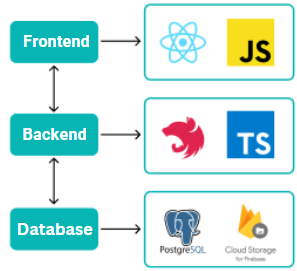
\includegraphics[width=6cm,height=6cm,keepaspectratio]{SWAReal.png}
  \end{center}
  \caption[โครงสร้างของเว็บไซต์]{โครงสร้างของเว็บไซต์}
  \label{fig:โครงสร้างของเว็บไซต์}
\end{figure}

\section{ฟีเจอร์}
\subsection{ฟีเจอร์การใช้งานของผู้เล่น}
การใช้งานในฝั่งผู้เล่นจะมีระบบหลักๆ ดังนี้
\begin{enumerate}
  \item ระบบสร้างทีม - ใช้สร้างทีมเพื่อเข้าร่วมการแข่งขันทัวร์นาเมนต์ต่างๆ โดยจะสร้างทีมเป็นของแต่ละเกมที่ต้องการแข่งแยกกัน เช่น ทีมValorant ก็จะใช้ลงทัวร์นาเมนต์ได้แค่เกม Valorant เท่านั้น
  \item ระบบจัดการทีม - ใช้จัดการคนในทีม รับคนเข้าทีม และแสดงประวัติการเล่นของทีม
  \item ระบบจัดการโปรไฟล์ - ใช้จัดการโปรไฟล์เปลี่ยนชื่อ แสดงข้อมูลการเข้าร่วมแข่งและทีม
  \item ระบบเลือก และสมัครทัวร์นาเมนต์ - เลือกทัวร์นาเมนต์ที่ต้องการแข่งขั้นสามารถดูรายละเอียด เลือกเกมที่ต้องการ และสมัครเข้าร่วมการแข่งขันได้
\end{enumerate}

\subsection{ฟีเจอร์การใช้งานของผู้จัดงาน}
การใช้งานในฝั่งผู้จัดการจะมีระบบหลักๆ ดังนี้
\begin{enumerate}
  \item ระบบสร้างจัดการทัวร์นาเมนต์ - ใช้สร้างทัวร์นาเมต์กำหนดรายระเอียดการแข่ง กฎกติกา เวลาแข่ง และรูปหน้าปกทัวร์นาเมนต์
  \item ระบบเดชบอร์ดในการจัดการทัวร์นาเมนต์ - ใช้ในการจัดการทัวร์นาเมนต์ผลแพ้ชนะ และคะแนน
  \item ระบบจัดตารางแข่ง - ใช้จัดการสายการแข่งโดยสามารถเลือกทีม และเวลาลงสายการแข่งได้ตามที่ต้องการ
\end{enumerate}

\section{ฐานข้อมูล}
ฐานข้อมูลที่ใช้ในโครงงานนี้จะมีด้วยกันทั้งหมด 9 tables ได้แก่
\begin{enumerate}
  \item User - ใช้ในการเก็บข้อมูลพื้นฐานของผู้ใช้
  \item Game - ใช้ในการเก็บข้อมูลเกมต่างๆเพื่อใช้เป็นข้อมูลในการสร้างทีม และทัวร์นาเมนต์
  \item Team - ใช้เก็บข้อมูล และรายเอียดของทีม
  \item Team Member - ใช้เก็บข้อมูลสมาชิกในทีมแต่ละทีม
  \item Team Request -  ใช้เก็บข้อมูลการขอเข้าสมัครเข้าร่วมทีมของแต่ละทีม
  \item Tournament - ใช้เก็บข้อมูล และรายละเอียดทัวร์นาเมนต์
  \item Tournament Join - ใช้เก็บข้อมูลทีมที่เข้าร่วมของแต่ละทัวร์นาเมนต์
  \item Match - ใช้เก็บข้อมูลเกมการแข่งขันว่าใครแข่งกับใครในแต่ละทัวร์นาเมนต์
  \item Match Results - ใช้เก็บข้อมูลผลการแข่งขันของแต่ละ Match
\end{enumerate}
\begin{figure}[h]
  \begin{center}
  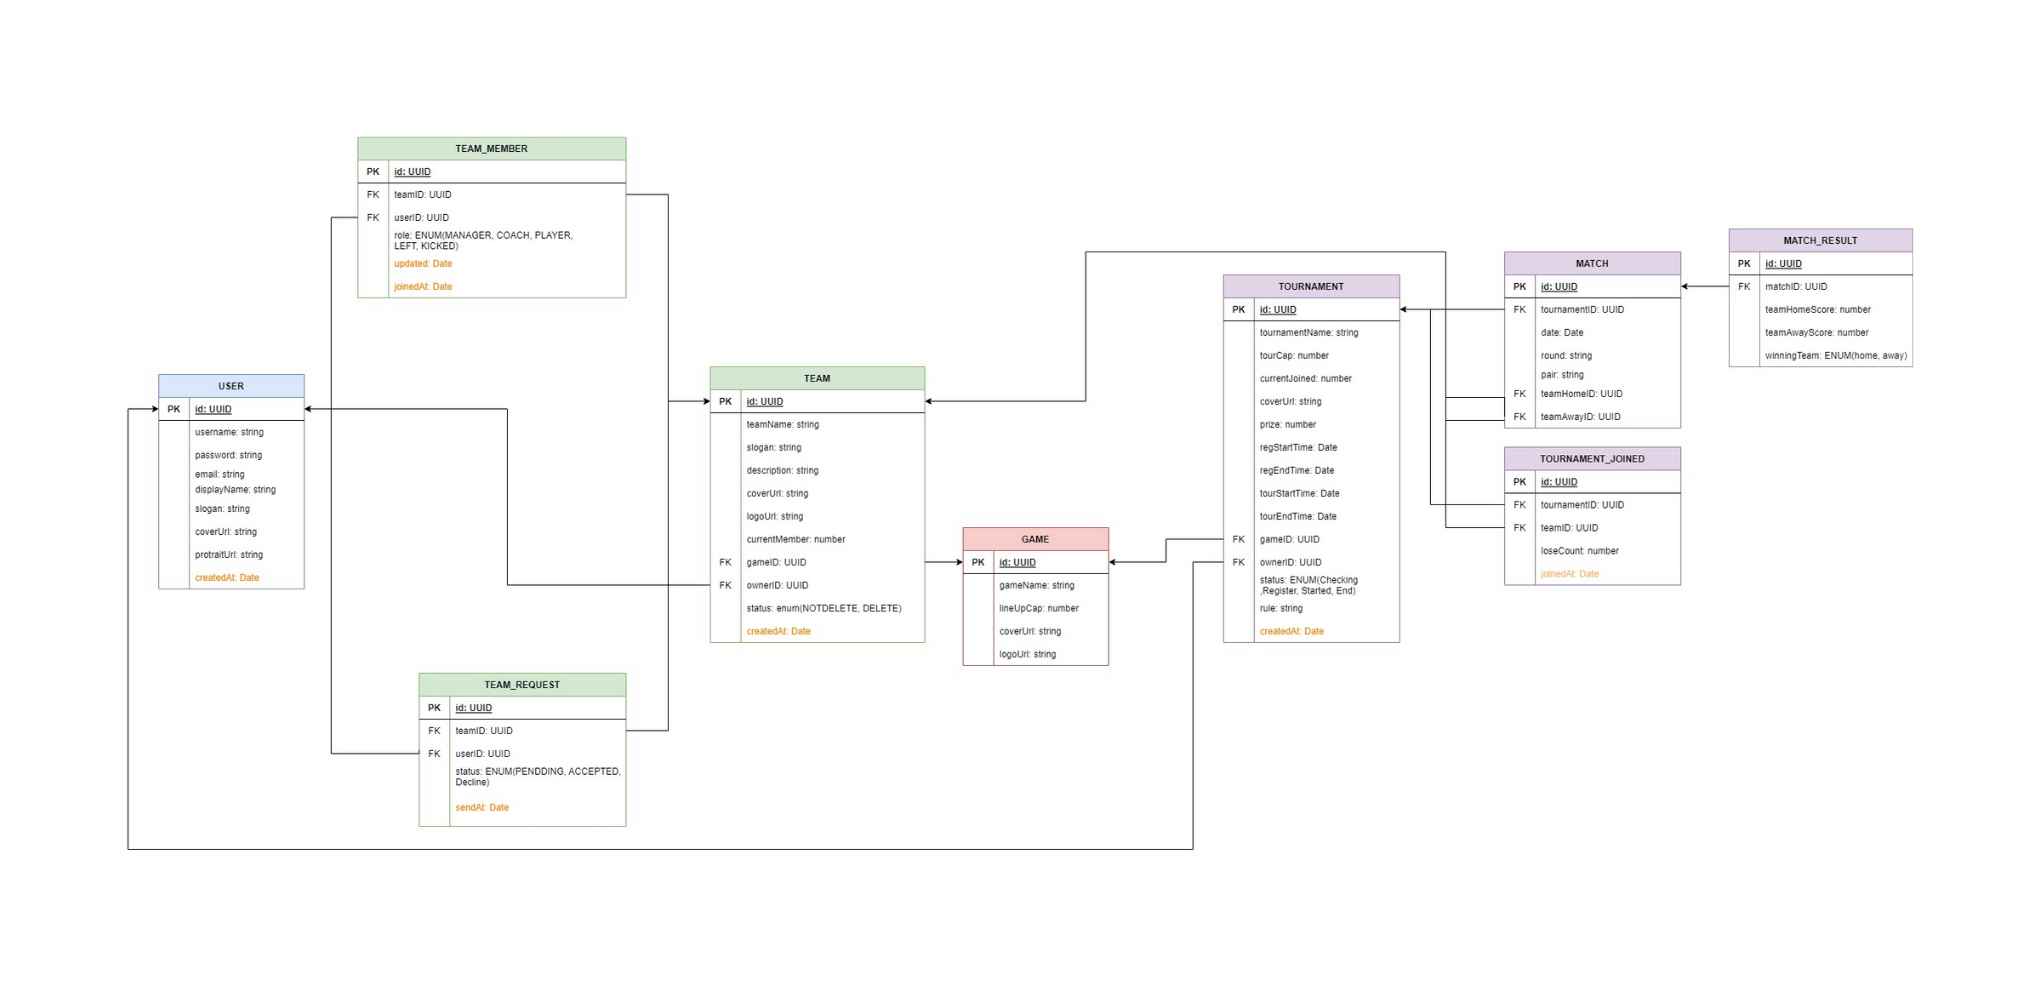
\includegraphics[width=18cm,height=6cm,keepaspectratio]{492_FyTy Tournament.png}
  \end{center}
  \caption[Database Schema]{Database Schema}
  \label{fig:Database Schema}
\end{figure}

\pagebreak

\section{authentication}
การที่จะเข้าถึง API Route ได้นั้นจะต้องมีการระบุตัวตนโดยใช้ JWT(JSON Web Token) โดยตัว JWT จะเข้ารหัสข้อมูลที่ส่งมาทำให้การส่งข้อมูลมีความปลอดภัย
โดยจะมีหลักการใช้งานดังนี้
\begin{enumerate}
  \item ผู้ใช้งานทำการ login เมื่อผู้ใช้งานทำการ login สำเร็จระบบจะนำ id ของ user ไปสร้าง token และส่งกลับไปยัง client
  \item ฝั่ง Client จะเซต Default การแนบ token มาด้วยทุกครั้งที่ทำการส่ง API Route มายัง server
  \item server จะตรวจเช็ค token ที่แนบมาก่อนว่า format ของ token เข้ารหัสถูกต้องหรือไม่ จาก secret key ที่เก็บไว้ในฝั่ง server หากถูกต้องจะทำการเข้าไปดูว่ามีข้อมูล user จริงหรือไม่จากค่า sub ที่แนบมากับ token
  \item เมื่อ token และ ข้อมูลถูกต้อง server จะคืนค่าข้อมูลจากฐานข้อมูลที่ต้องการให้
\end{enumerate}


\section{อินเตอร์เฟส และการทำงาน}
\subsection{หน้าโฮม}
เป็นหน้าแรกหลังจากเขามาในเว็ปไซต์โดยจะมี navbar ด้านบนใช้ในการนำทางไปในหน้าที่ต้องการ
แต่การที่จะไปหน้าอื่นได้นั้นต้องทำการ login ก่อนถึงจะสามารถไปได้โดยการ login นั้นสามารถใช้บัญชีที่สมัครกับทางเว็ปไซต์ได้ หรือจะใช้บัญชี Google ก็สามารถทำได้
\subsection{หน้าเดชบอร์ดทีม}
เป็นหน้าที่ใช้ในการค้นหาทีมโดยจะมีระบบในการค้นหาทีม และการกรองโดยสามารถกดเลือกจากการ์ดเกมต่างๆ หรือช่องค้นหาได้ และใช้ในการสร้างทีมโดยการสร้างทีมสามารถอัพโหลดรูปโลโก้ทีม และรูปปกทีมได้ตามความต้องการ
\subsection{หน้ารายละเอียดทีม}
เป็นหน้าที่จะบอกรายละเอียดของทีมนั้นว่าเคยไปแข่งทัวร์นาเมนต์อะไรไปแล้วบ้าง และมีสมาชิกในทีมเป็นใครบ้าง โดยแต่การ์ดที่แสดงรายละเอียดจะสามารถคลิกไปดูรายละเอียดได้โดยระบบจะทำการนำทางไปยังหน้าของรายละเอียดนั้นๆ
และถ้าหากเป็นเจ้าของทีมจะสามารถแก้ไขรูปทีม และรูปปกทีมได้
\subsection{หน้าแดชบอร์ดทัวร์นาเมนต์}
เป็นหน้าที่ใช้ในการค้นหาทีมโดยจะมีระบบในการค้นหาทัวร์นาเมนต์และการกรองโดยสามารถกดเลือกจากการ์ดเกมต่างๆ หรือช่องค้นหาได้ และใช้ในการสร้างทีมโดยการสร้างทีมสามารถอัพโหลดรูปโลโก้ทีม และรูปปกทีมได้ตามความต้องการ
\subsection{หน้ารายละเอียดทัวร์นาเมนต์}
เป็นหน้าที่จะแสดงรายละเอียดต่างๆของทัวร์นาเมนต์เช่น รายละเอียดเงินรางวัล เวลาแข่ง กฎกติกาการแข่ง ตารางเเข่ง และมีทีมอะไรบ้างที่เคยเข้าไปร่วมทีมด้วย
และถ้าหากเป็นเจ้าของทัวร์นาเมนต์เราจะสามารถแก้ไขภาพปกของทัวร์นาเมนต์ กฎกติกา จัดผู้เล่นลงสายได้ และสถานะของทัวร์นาเมนต์(register, start, end)
\subsection{หน้าสร้างทัวร์นาเมนต์}
เป็นหน้าที่แสดงทัวร์นาเมนต์ที่เราได้สร้างไปทั้งที่ยังดำเนินการอยู่ และที่จบไปแล้ว และเราสามารถสร้างทัวร์นาเมนต์ได้โดยกดไปที่ปุ่ม Create จากนั้นจะมี popup ขึ้นมาให้กรอกรายละเอียดเมื่อกรอกรายละเอียดเสร็จเรียบร้อยแล้วระบบจะนำทางไปยังหน้ารายละเอียดทัวร์นาเมนต์เพื่อใส่รายละเอียดเพิ่มเติมก่อนที่จะ public ทัวร์นาเมนต์นี้ให้ผู้อื่นสมัคร
\subsection{หน้าโปรไฟล์}
เป็นหน้าที่จะบอกรายละเอียดของผู้ใช้คนนั้นว่าเคยไปแข่งทัวร์นาเมนต์อะไรไปแล้วบ้าง และมีทีมอะไรบ้างที่เคยเข้าไปร่วมทีมด้วย โดยแต่การ์ดที่แสดงรายละเอียดจะสามารถคลิกไปดูรายละเอียดได้โดยระบบจะทำการนำทางไปยังหน้าของรายละเอียดนั้นๆ
และถ้าหากเป็นเจ้าของทีมจะสามารถแก้ไขรูปโปรไฟล์ และรูปปกได้
\subsection{หน้าตารางเวลาแข่ง}
เป็นหน้าที่จะแสดงเวลาการแข่งที่กำลังจะมาถึงโดยจะเรียงจากเวลาที่ใกล้ที่สุดก่อน และเมื่อเวลาผ่านไปจะถูกนำออกไม่นำมาแสดง


%  home
    \begin{figure}[ht]
      \begin{center}
      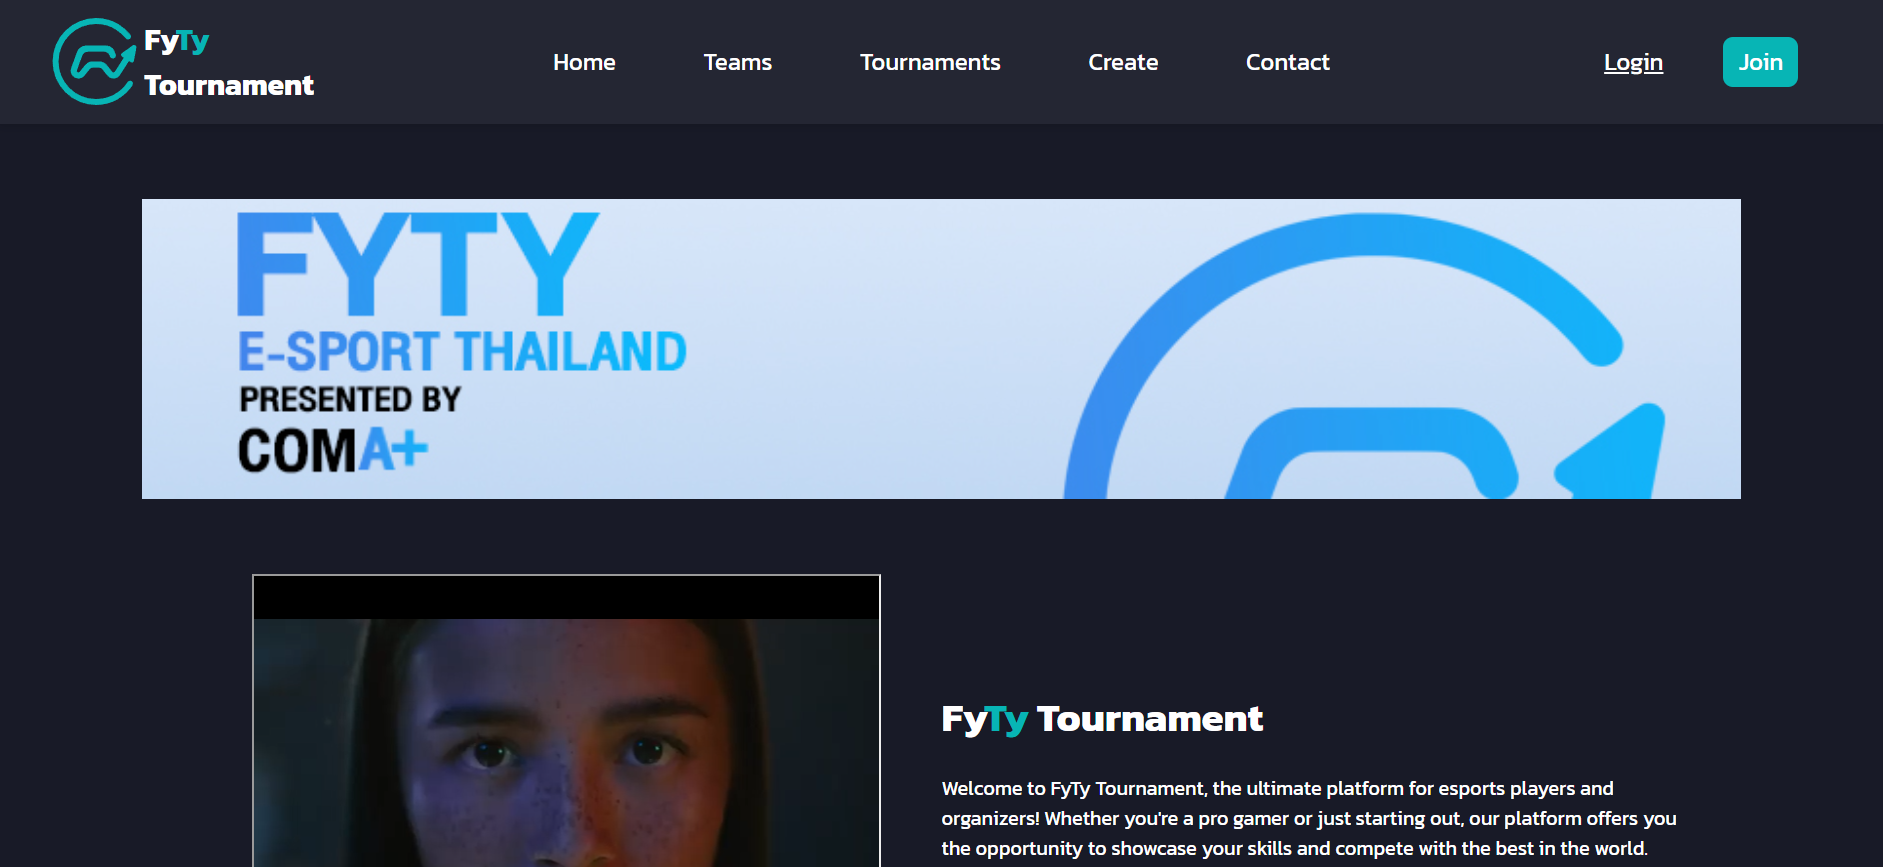
\includegraphics[width=18cm,height=7cm,keepaspectratio]{home_no_login.png}
      \end{center}
      \caption[หน้าโฮม]{หน้าโฮม}
      \label{fig:หน้าโฮม}
    \end{figure}
    \begin{figure}[ht]
      \begin{center}
        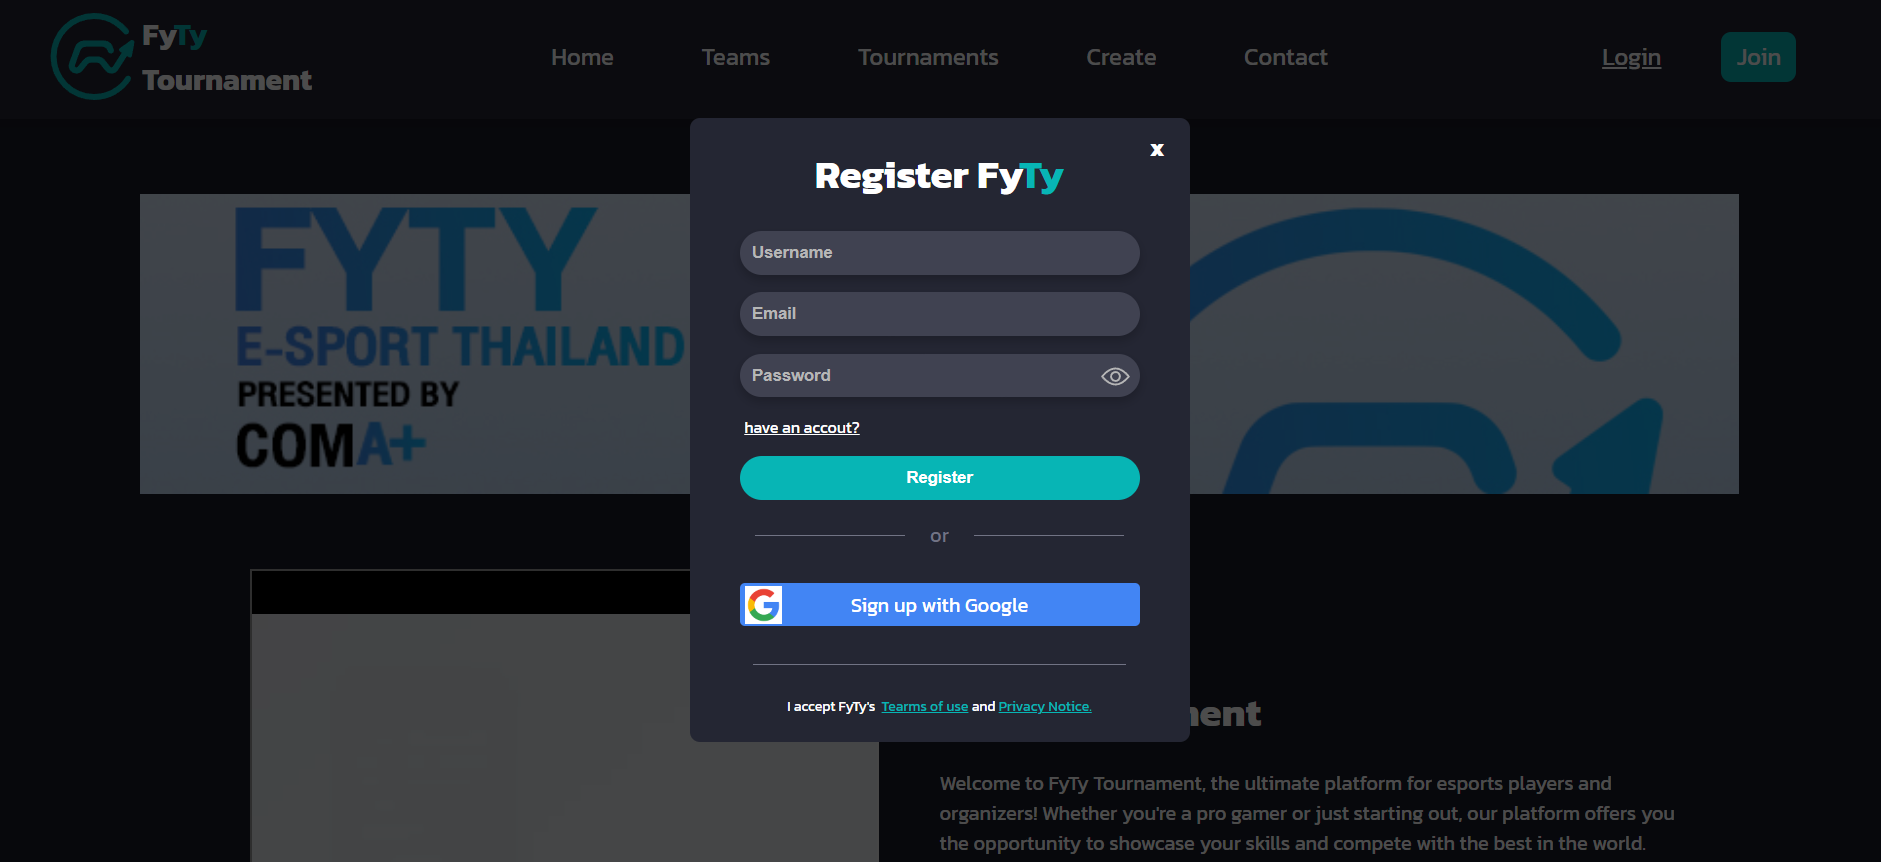
\includegraphics[width=18cm,height=7cm,keepaspectratio]{register.png}
      \end{center}
      \caption[Register Popup]{Register Popup}
      \label{fig:Register Popup}
    \end{figure}
    \begin{figure}[ht]
      \begin{center}
        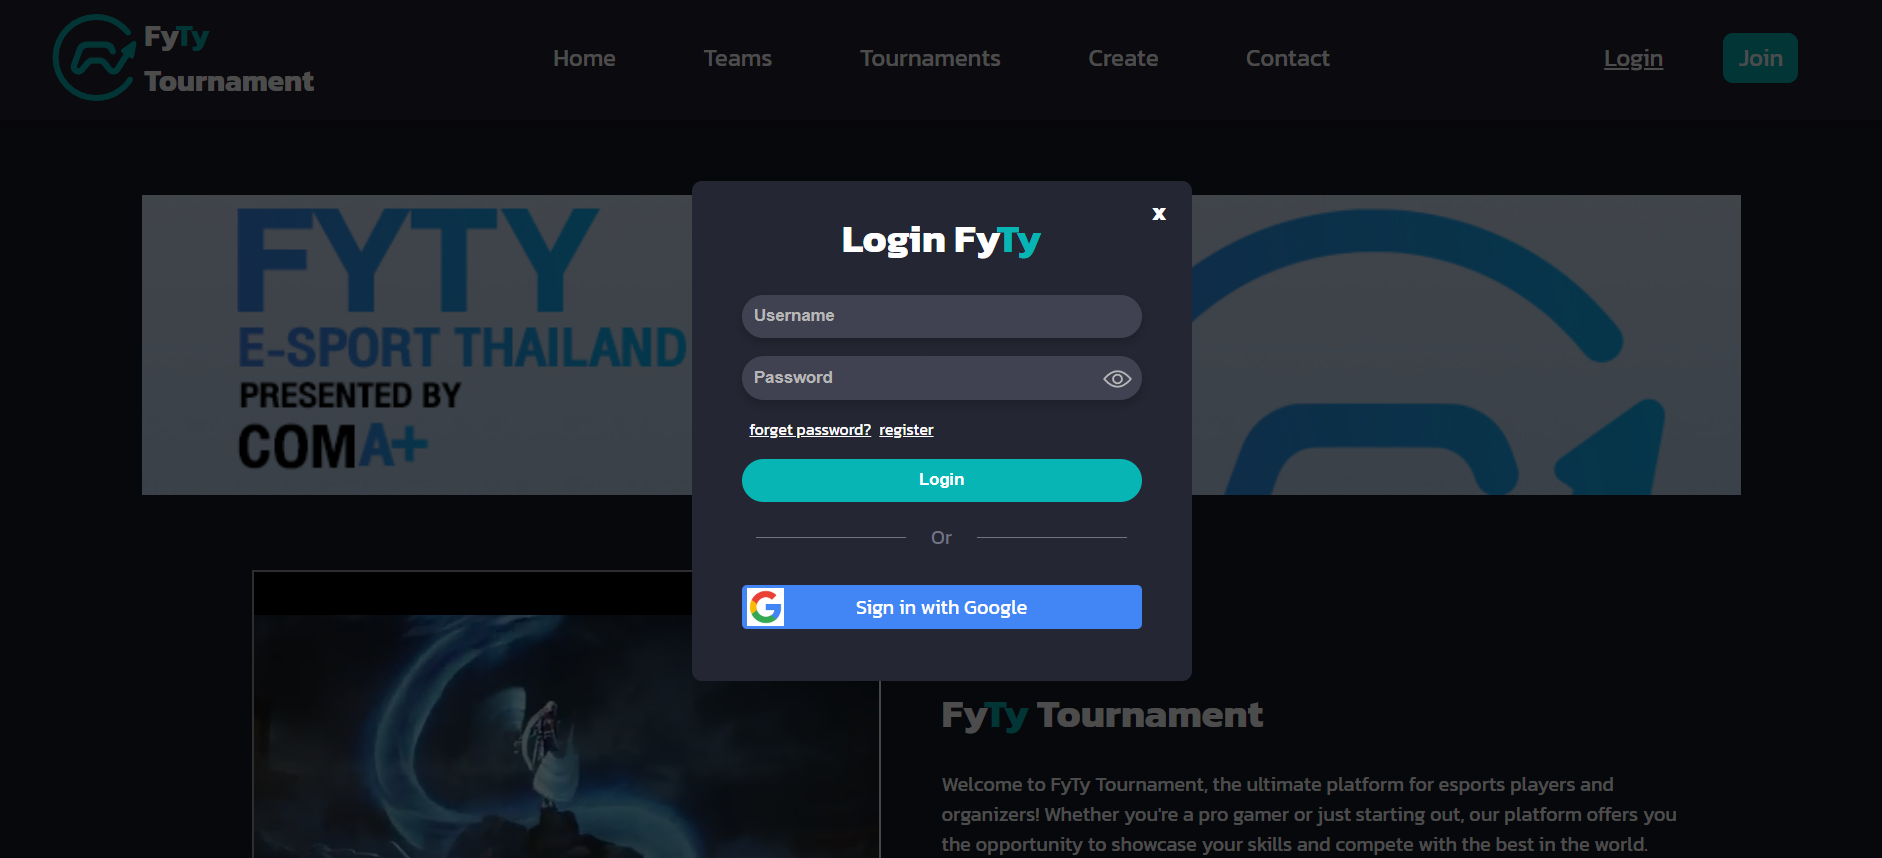
\includegraphics[width=18cm,height=7cm,keepaspectratio]{login.png}
      \end{center}
      \caption[Login Popup]{Login Popup}
      \label{fig:Login Popup}
    \end{figure}
    \begin{figure}[ht]
      \begin{center}
      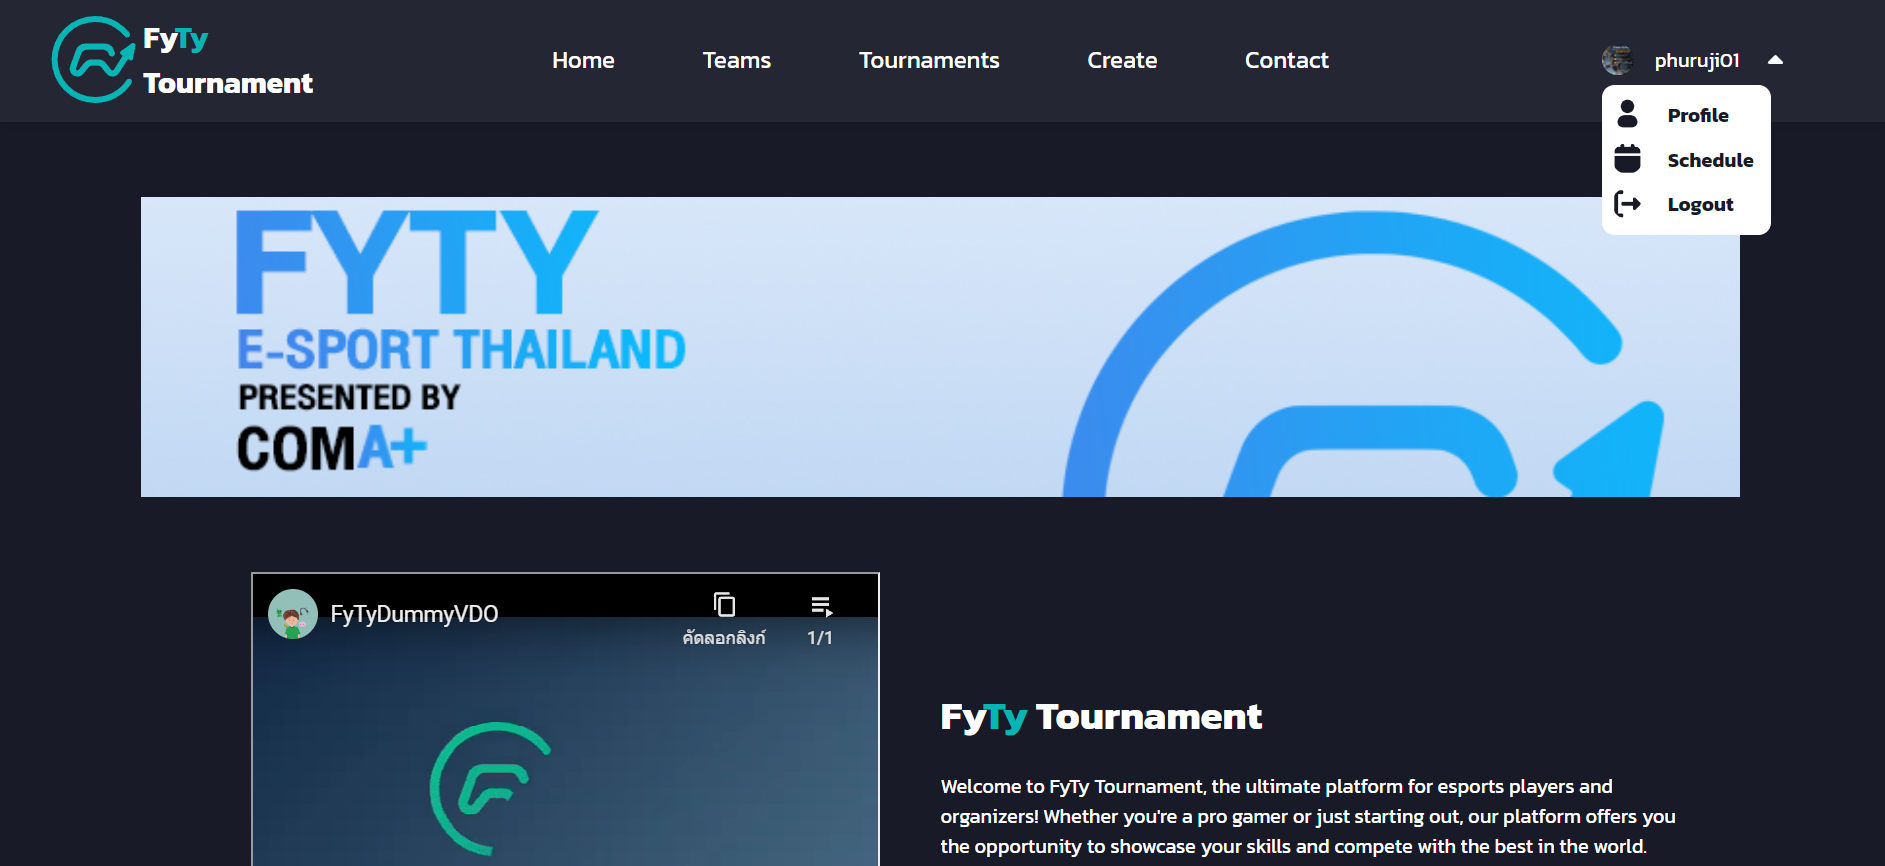
\includegraphics[width=18cm,height=7cm,keepaspectratio]{home_full.png}
      \end{center}
      \caption[หน้าโฮมหลังจาก Login]{หน้าโฮมหลังจาก Login}
      \label{fig:หน้าโฮมหลังจาก Login}
    \end{figure}
    \begin{figure}[ht]
      \begin{center}
      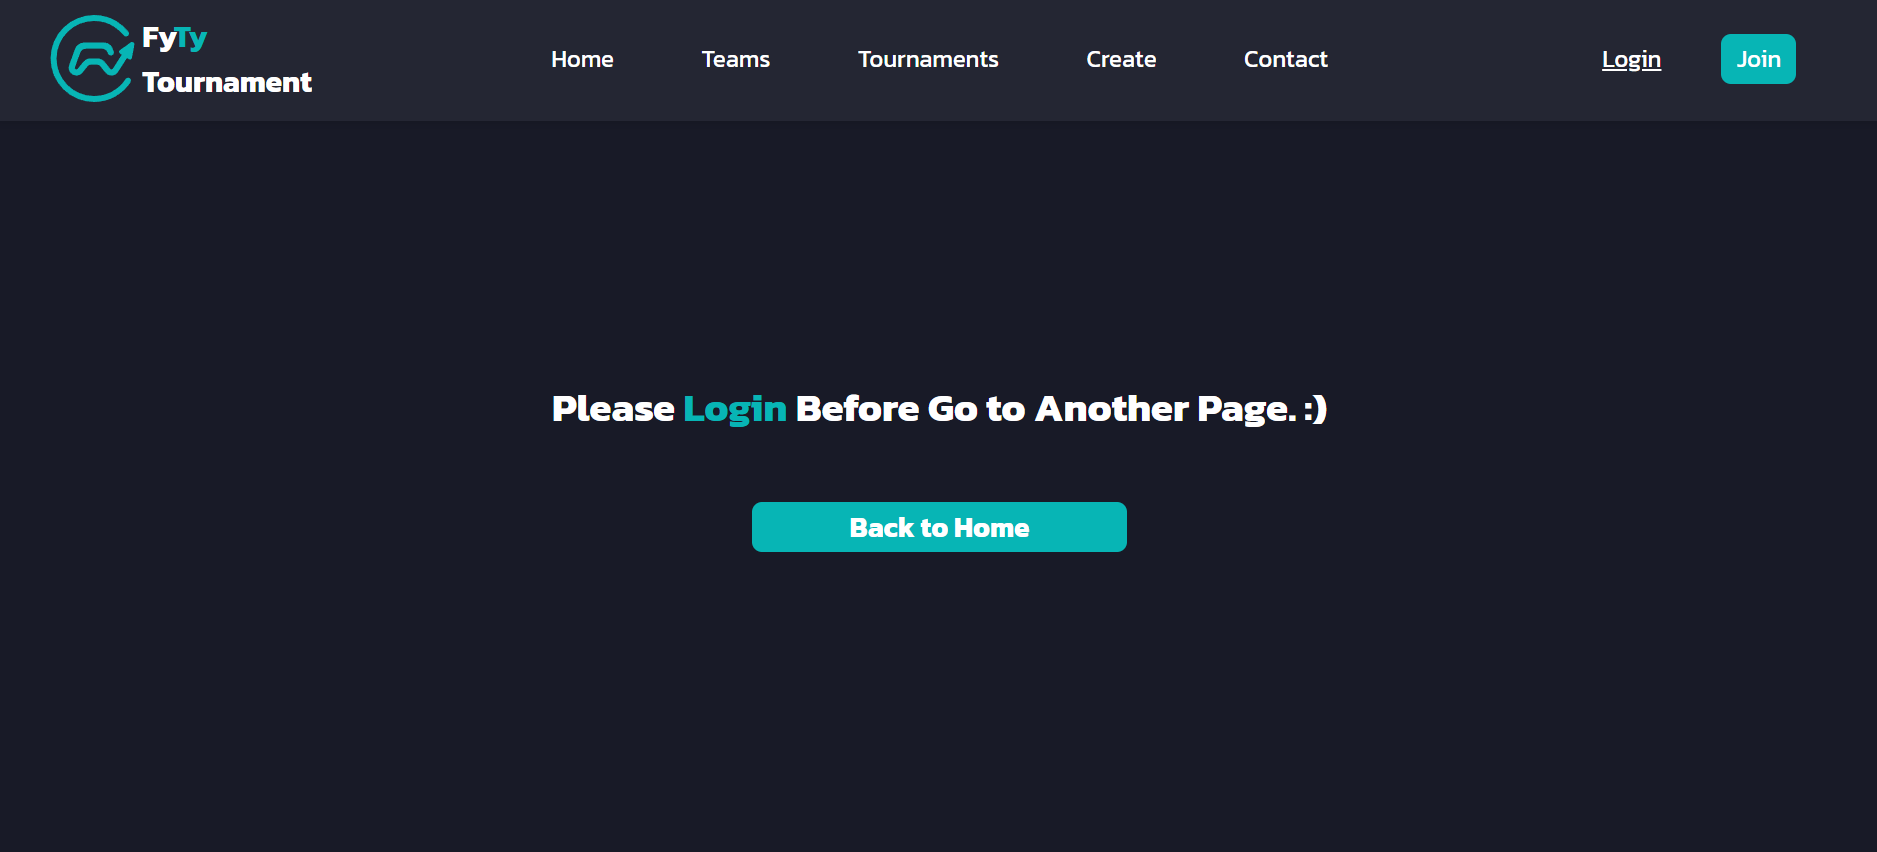
\includegraphics[width=18cm,height=7cm,keepaspectratio]{un_auth.png}
      \end{center}
      \caption[หน้าแจ้งเตือนหากไม่ได้ Login]{หน้าแจ้งเตือนหากไม่ได้ Login}
      \label{fig:หน้าแจ้งเตือนหากไม่ได้ Login}
    \end{figure}

    % team
    \begin{figure}[ht]
      \begin{center}
      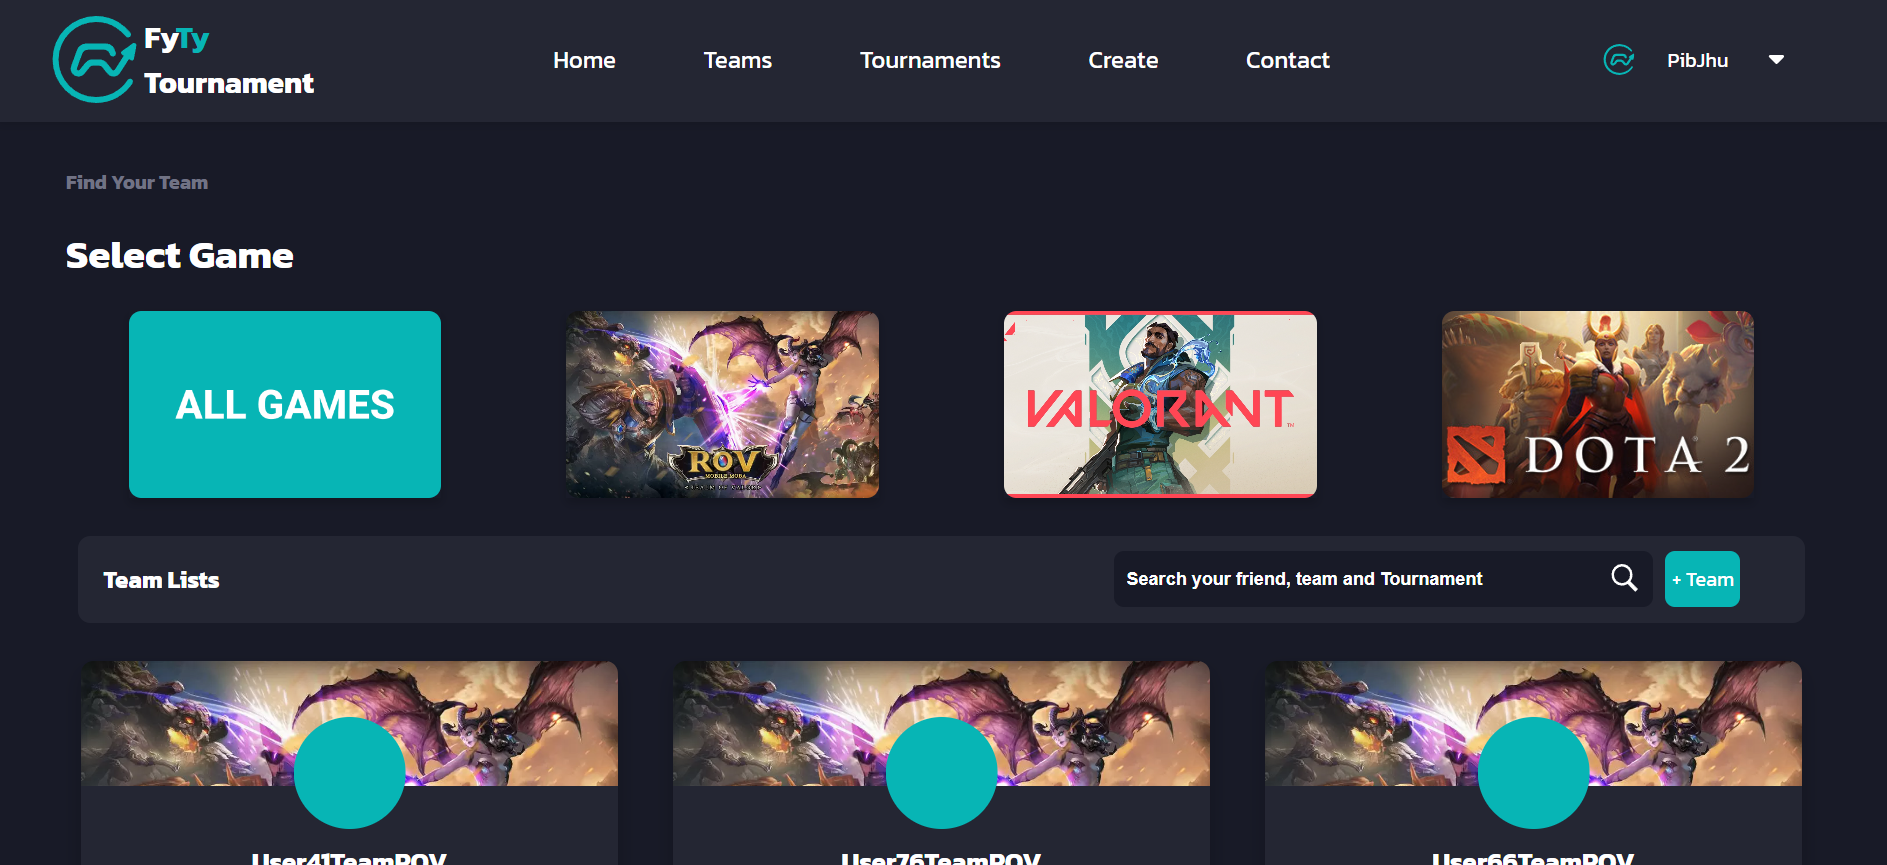
\includegraphics[width=18cm,height=7cm,keepaspectratio]{team.png}
      \end{center}
      \caption[หน้าเดชบอร์ดทีม]{หน้าเดชบอร์ดทีม}
      \label{fig:หน้าเดชบอร์ดทีม}
    \end{figure}
    \begin{figure}[ht]
      \begin{center}
      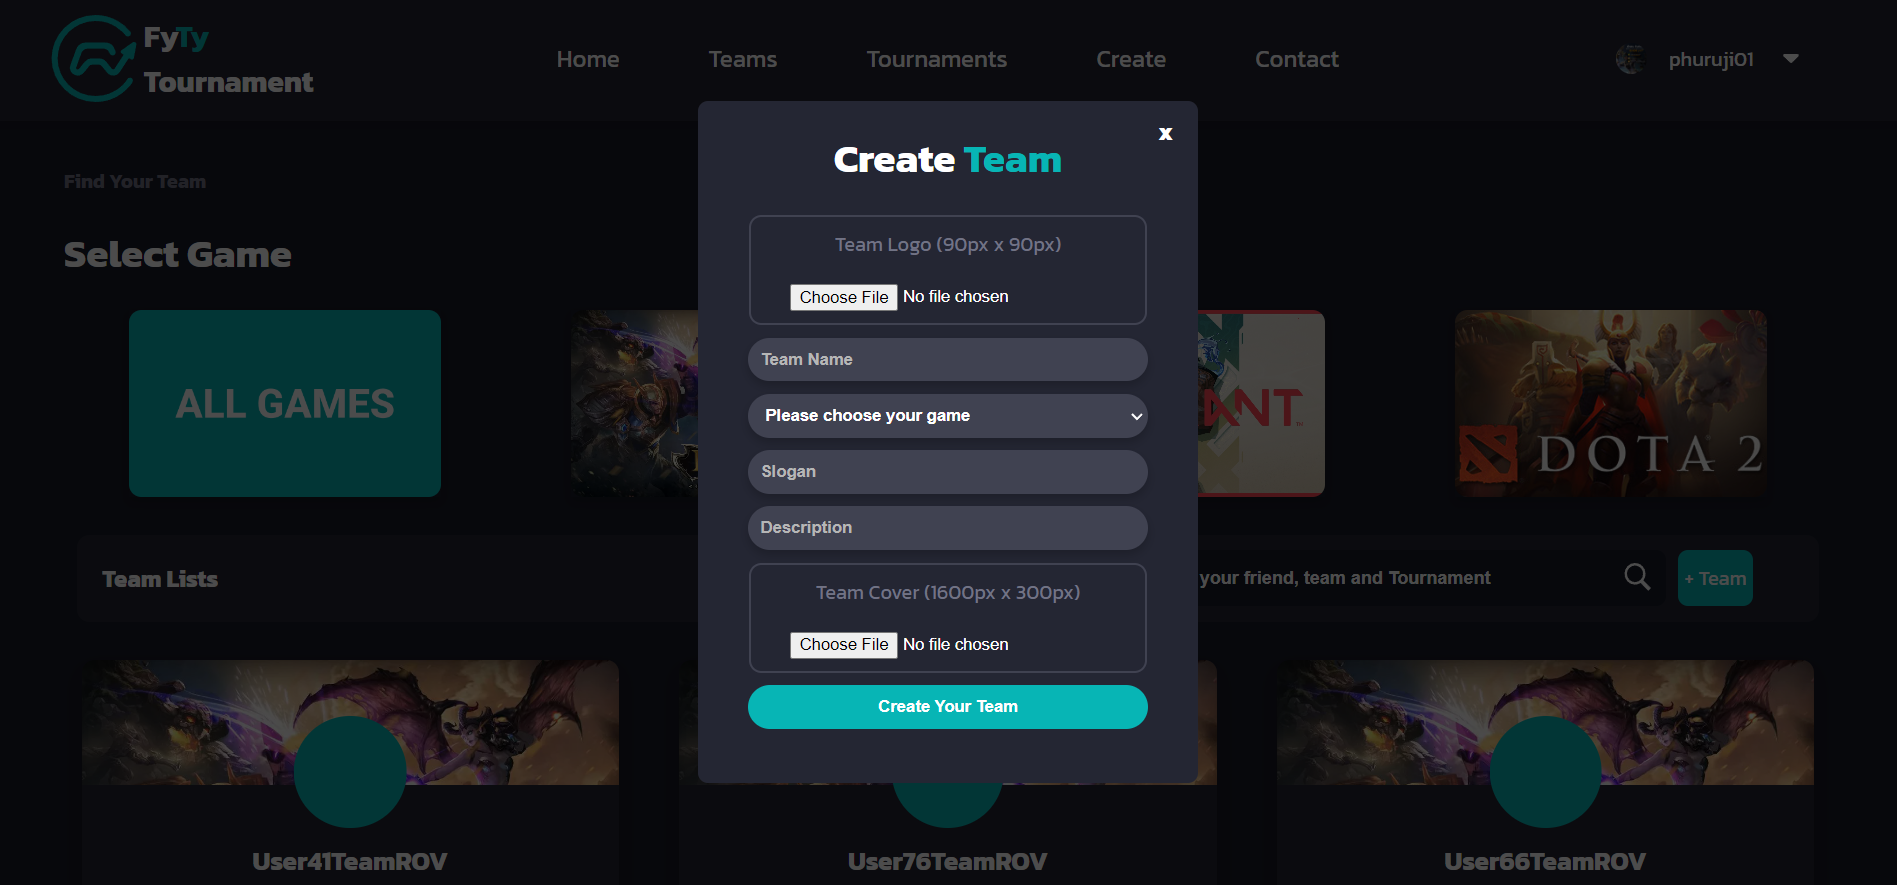
\includegraphics[width=18cm,height=7cm,keepaspectratio]{team_create.png}
      \end{center}
      \caption[Create Team Popup]{Create Team Popup}
      \label{fig:Create Team Popup}
    \end{figure}

    % team each
    \begin{figure}[ht]
      \begin{center}
      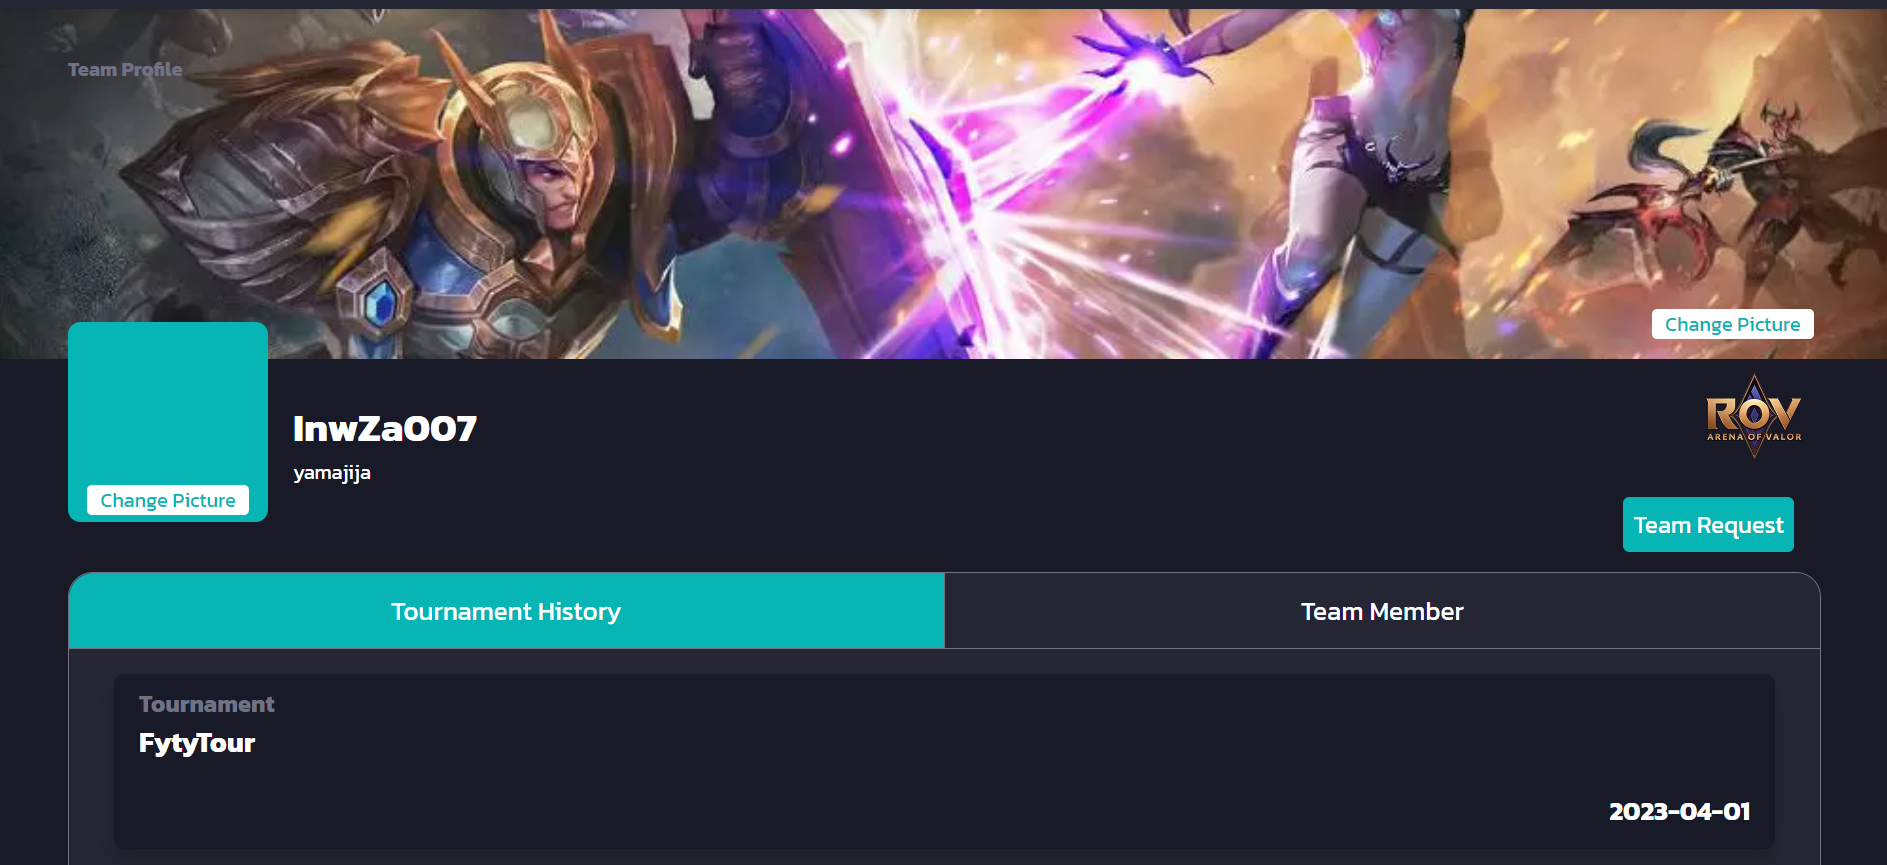
\includegraphics[width=18cm,height=7cm,keepaspectratio]{team_each_th.png}
      \end{center}
      \caption[หน้ารายละเอียดทีม และประวัติการแข่งขัน]{หน้ารายละเอียดทีม และประวัติการแข่งขัน}
      \label{fig:หน้ารายละเอียดทีม และประวัติการแข่งขัน}
    \end{figure}
    \begin{figure}[ht]
      \begin{center}
      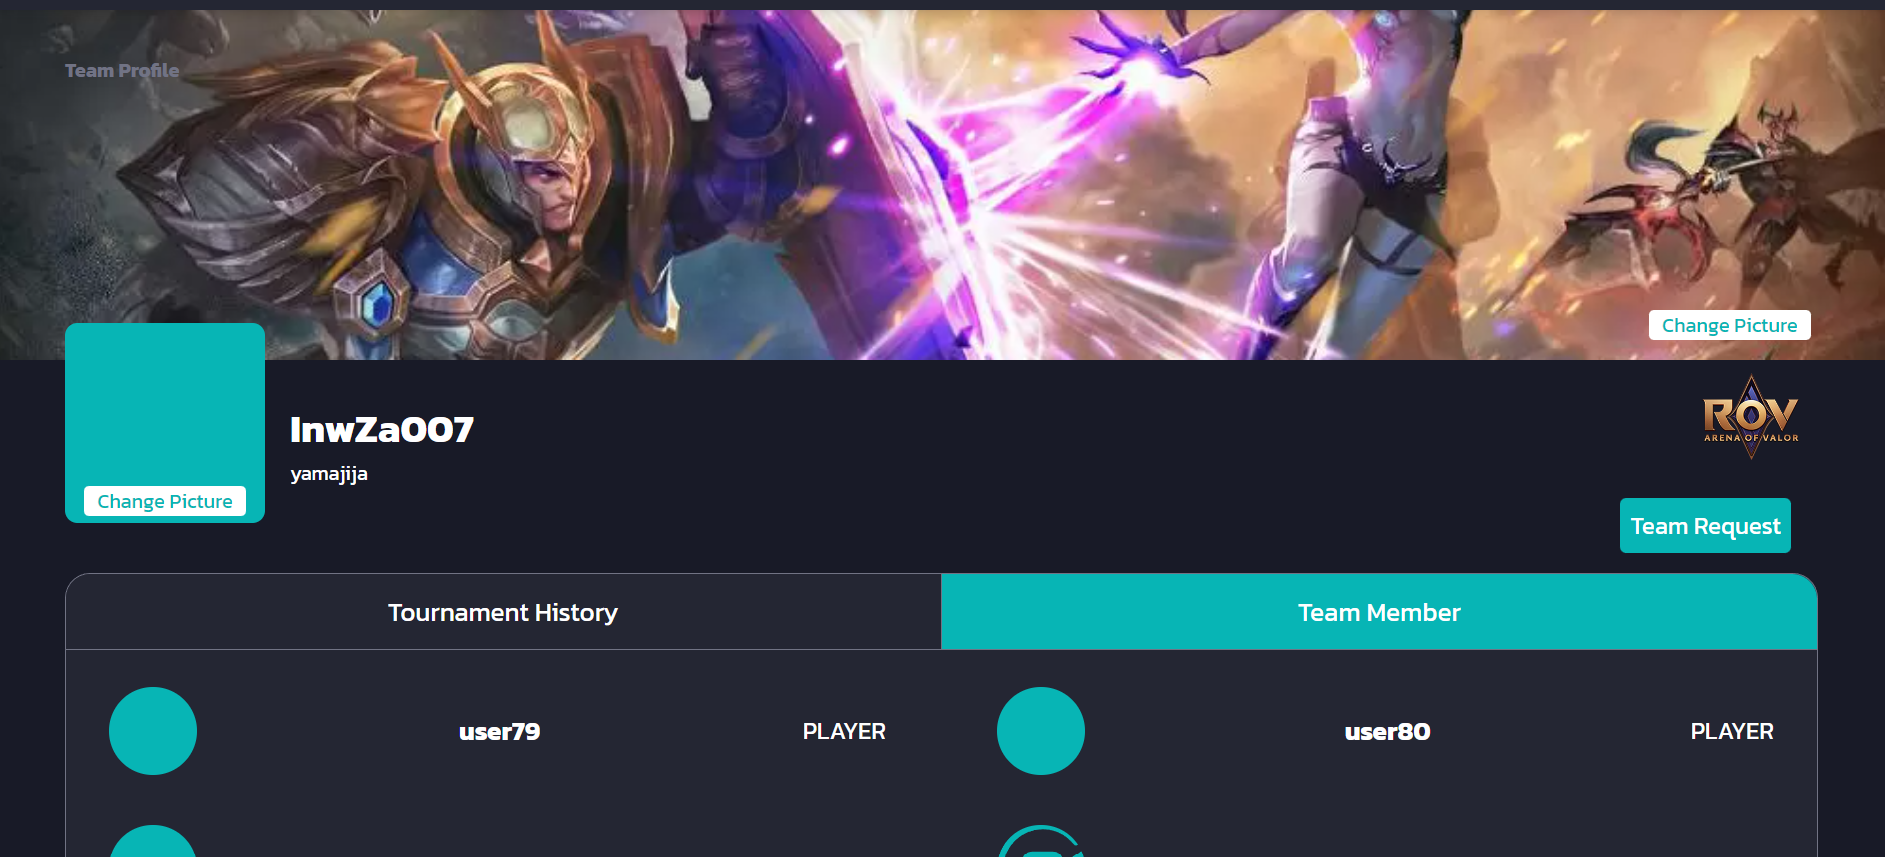
\includegraphics[width=18cm,height=7cm,keepaspectratio]{team_each_tm.png}
      \end{center}
      \caption[หน้ารายละเอียดทีม และสมาชิกทีม]{หน้ารายละเอียดทีม และสมาชิกทีม}
      \label{fig:หน้ารายละเอียดทีม และสมาชิกทีม}
    \end{figure}
    \begin{figure}[ht]
      \begin{center}
      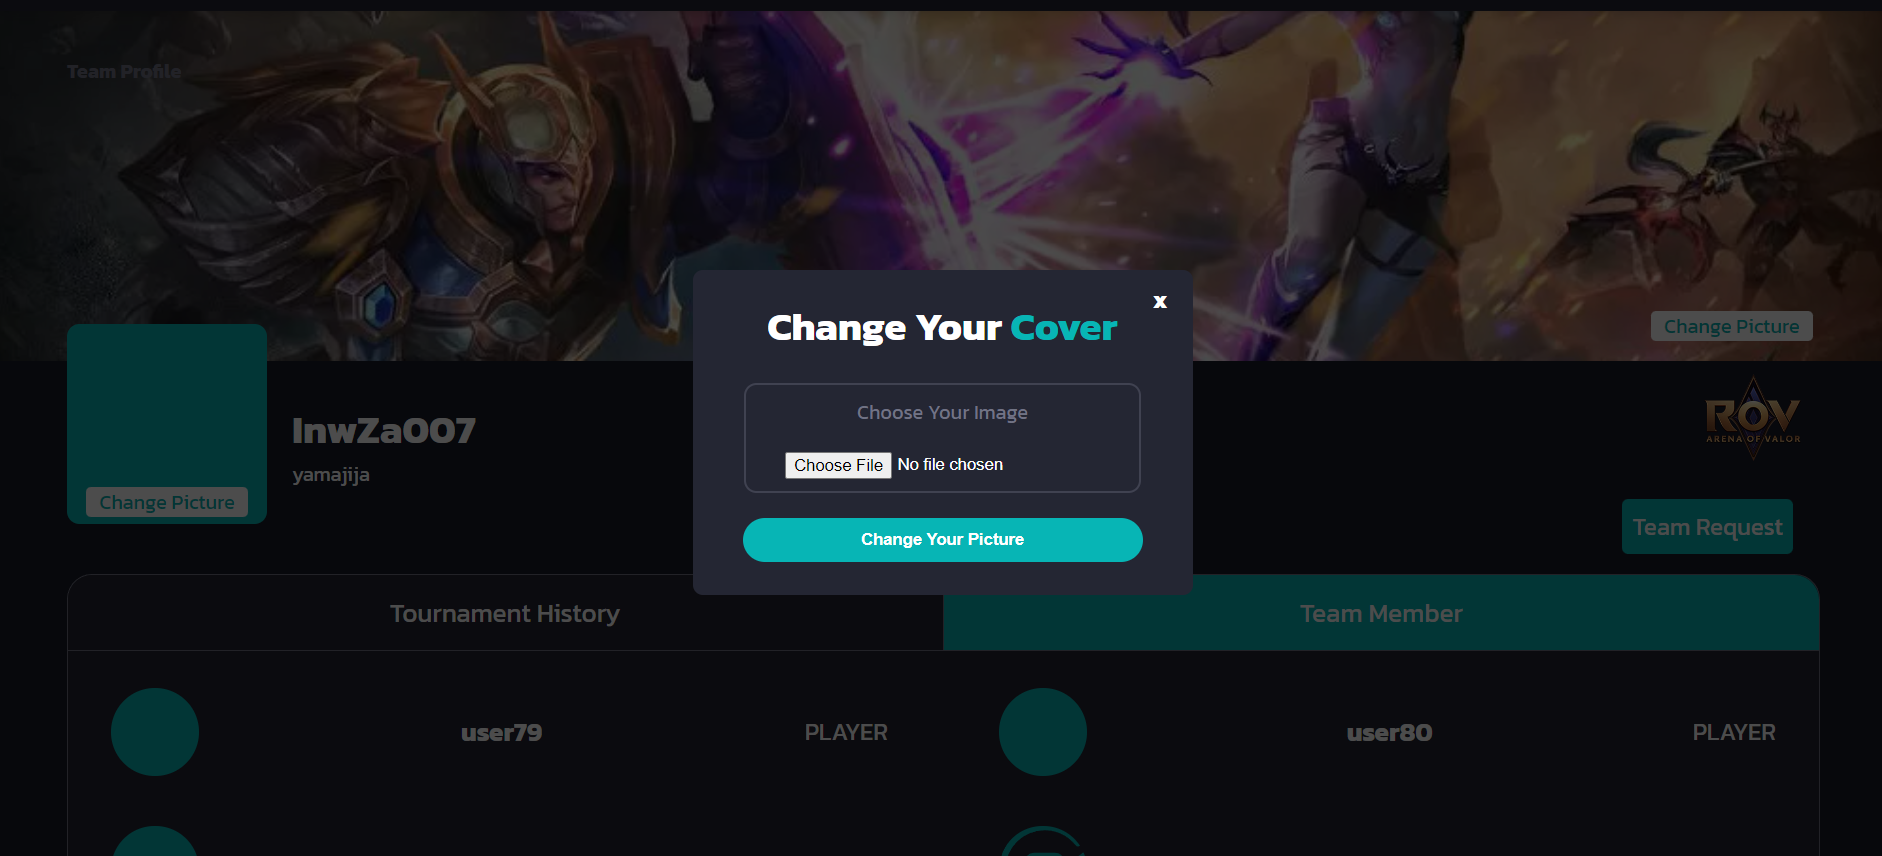
\includegraphics[width=18cm,height=7cm,keepaspectratio]{team_each_change_pic.png}
      \end{center}
      \caption[Create Picture Popup]{Create Picture Popup}
      \label{fig:Change Picture Popup}
    \end{figure}

    % tournmanet
    \begin{figure}[ht]
      \begin{center}
      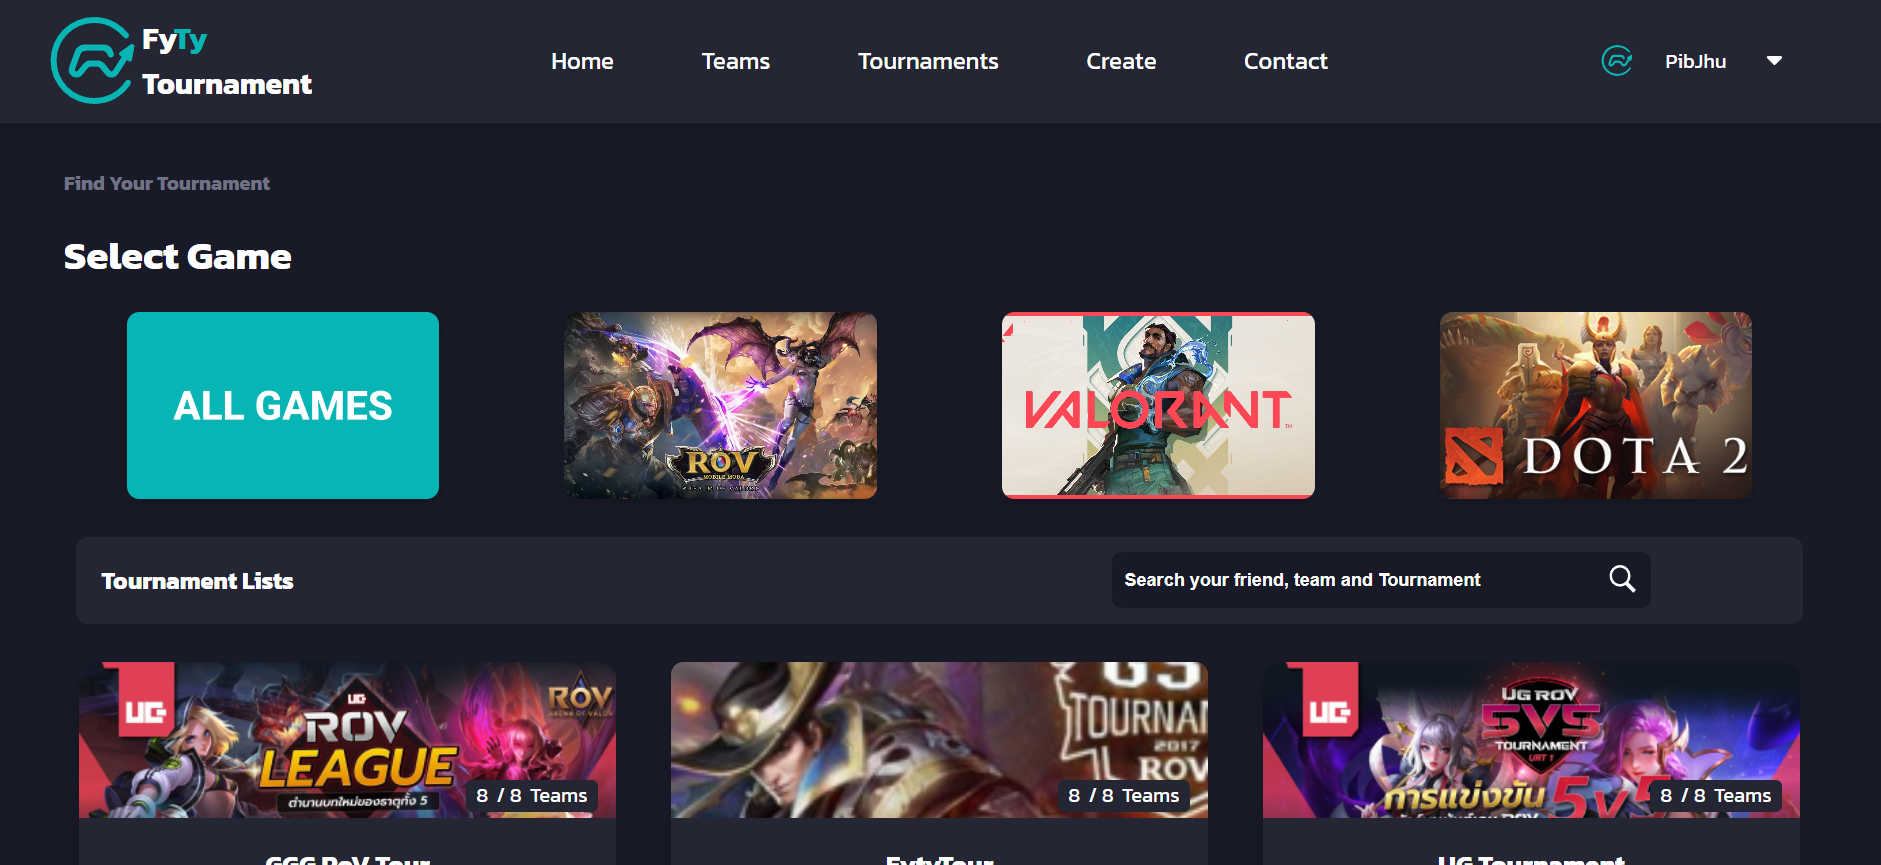
\includegraphics[width=18cm,height=7cm,keepaspectratio]{tournament.png}
      \end{center}
      \caption[หน้าแดชบอร์ดทัวร์นาเมนต์]{หน้าแดชบอร์ดทัวร์นาเมนต์}
      \label{fig:หน้าแดชบอร์ดทัวร์นาเมนต์}
    \end{figure}
    % tournament each
    \begin{figure}[ht]
      \begin{center}
      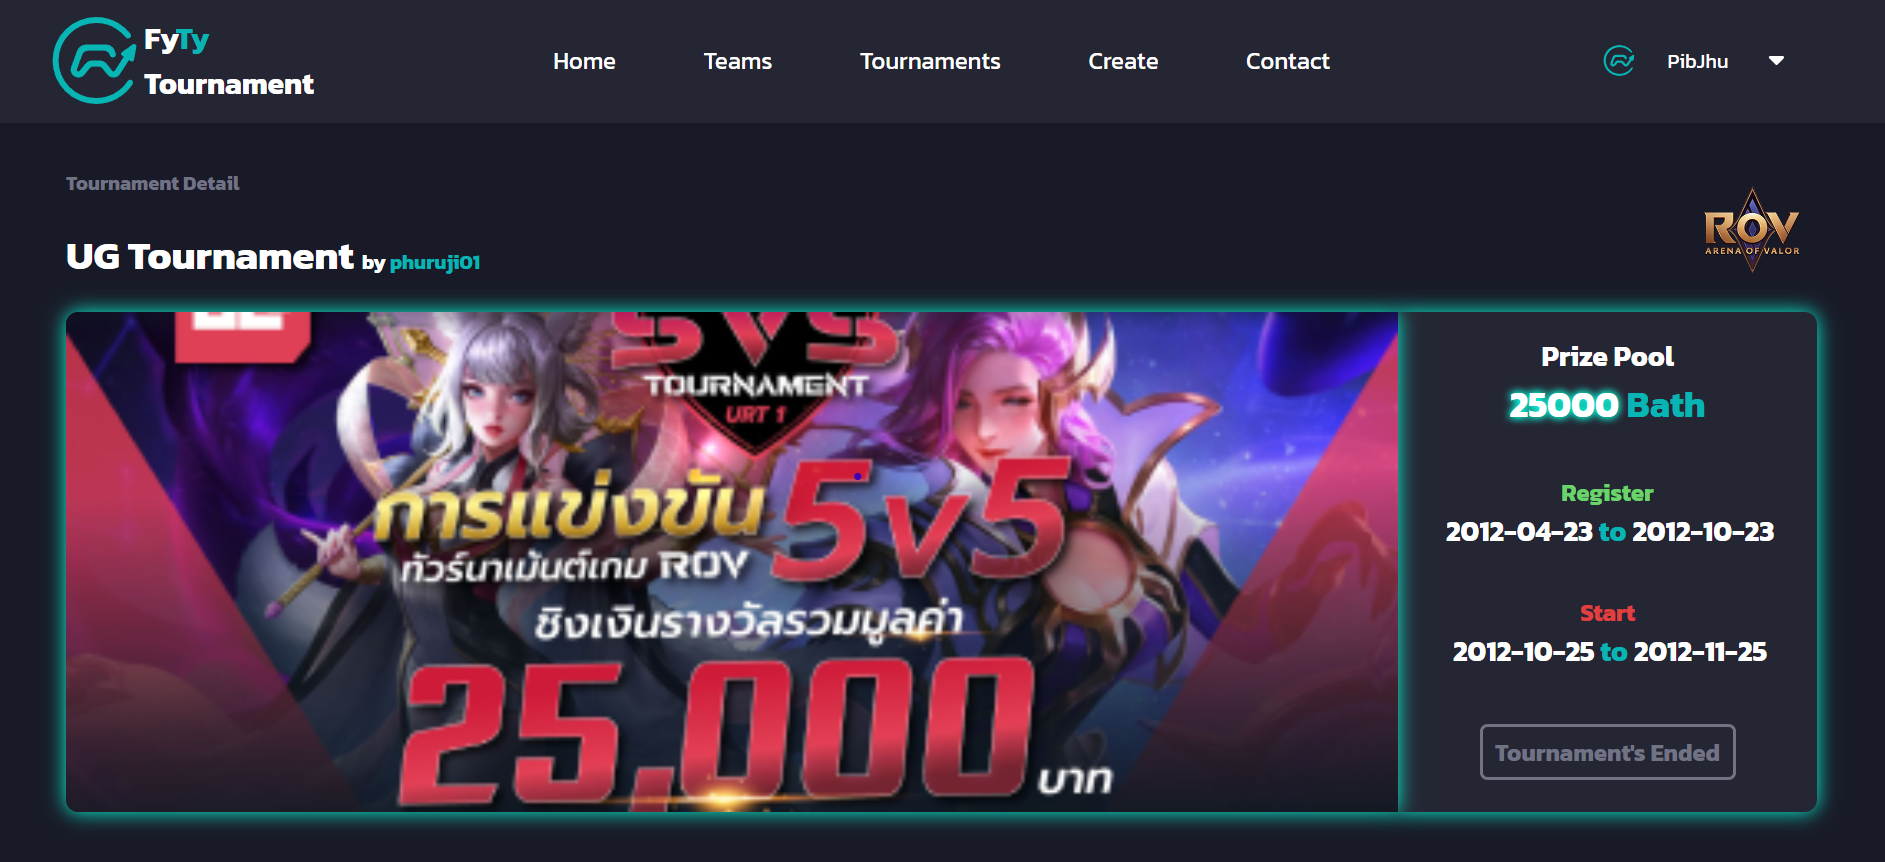
\includegraphics[width=18cm,height=7cm,keepaspectratio]{tournament_each_detail.png}
      \end{center}
      \caption[หน้ารายละเอียดทัวร์นาเมนต์(รายละเอียดทัวร์นาเมนต์)]{หน้ารายละเอียดทัวร์นาเมนต์(รายละเอียดทัวร์นาเมนต์)}
      \label{fig:หน้ารายละเอียดทัวร์นาเมนต์(รายละเอียดทัวร์นาเมนต์)}
    \end{figure}
    \begin{figure}[ht]
      \begin{center}
      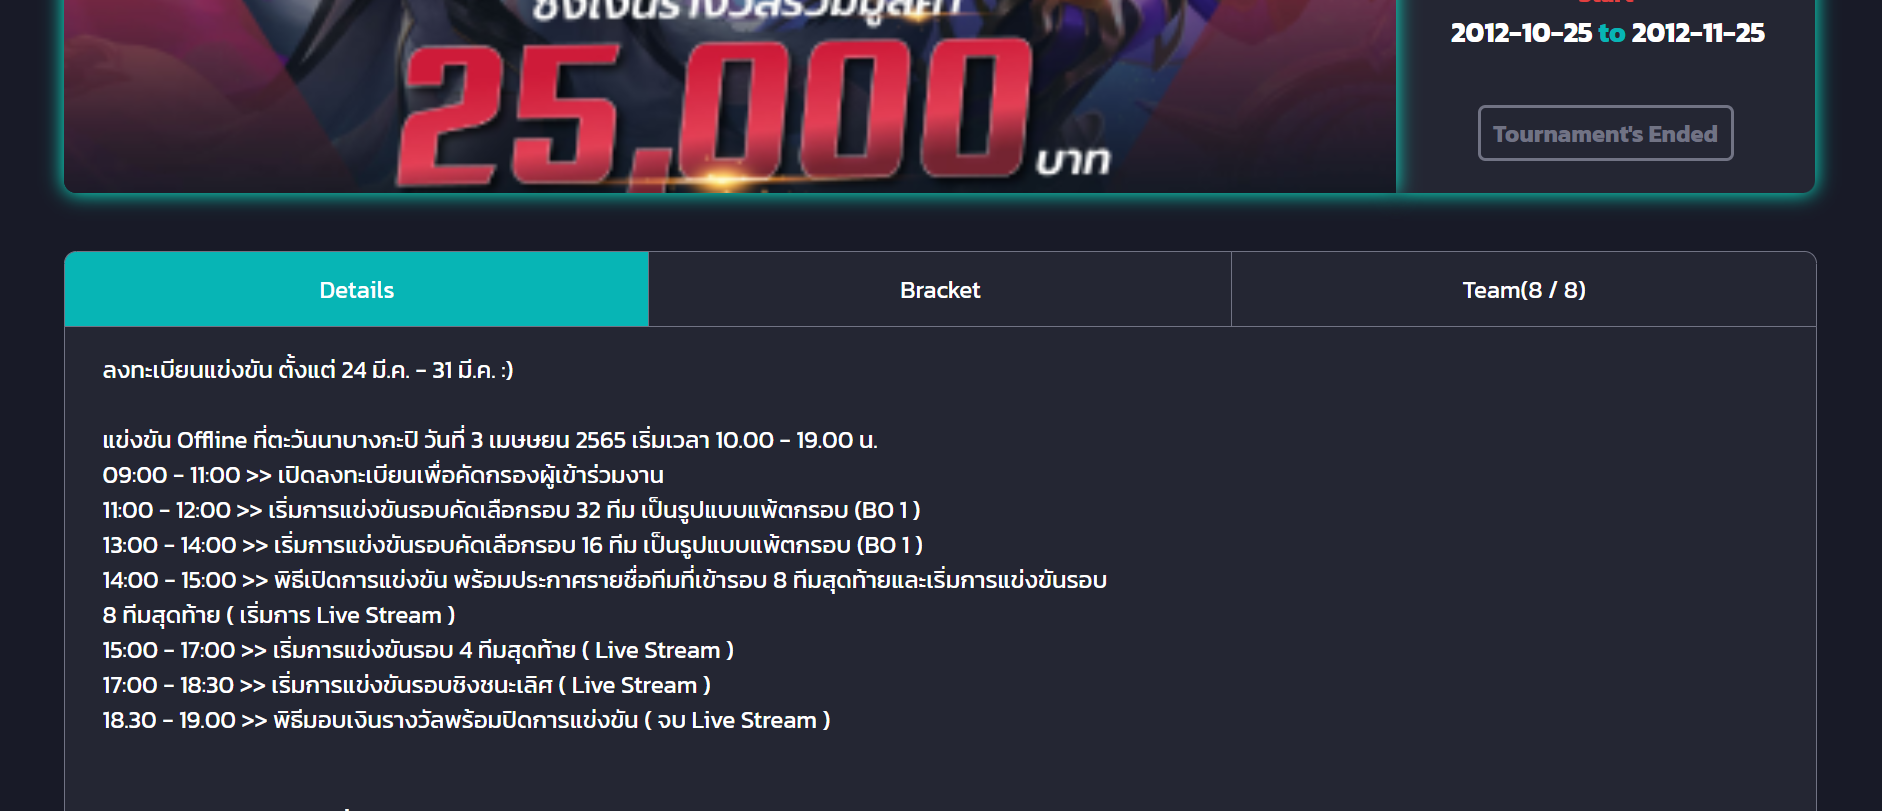
\includegraphics[width=18cm,height=7cm,keepaspectratio]{tournament_each_rule.png}
      \end{center}
      \caption[หน้ารายละเอียดทัวร์นาเมนต์(รายละเอียดการแข่ง)]{หน้ารายละเอียดทัวร์นาเมนต์(รายละเอียดการแข่ง)}
      \label{fig:หน้ารายละเอียดทัวร์นาเมนต์(รายละเอียดการแข่ง)}
    \end{figure}
    \begin{figure}[ht]
      \begin{center}
      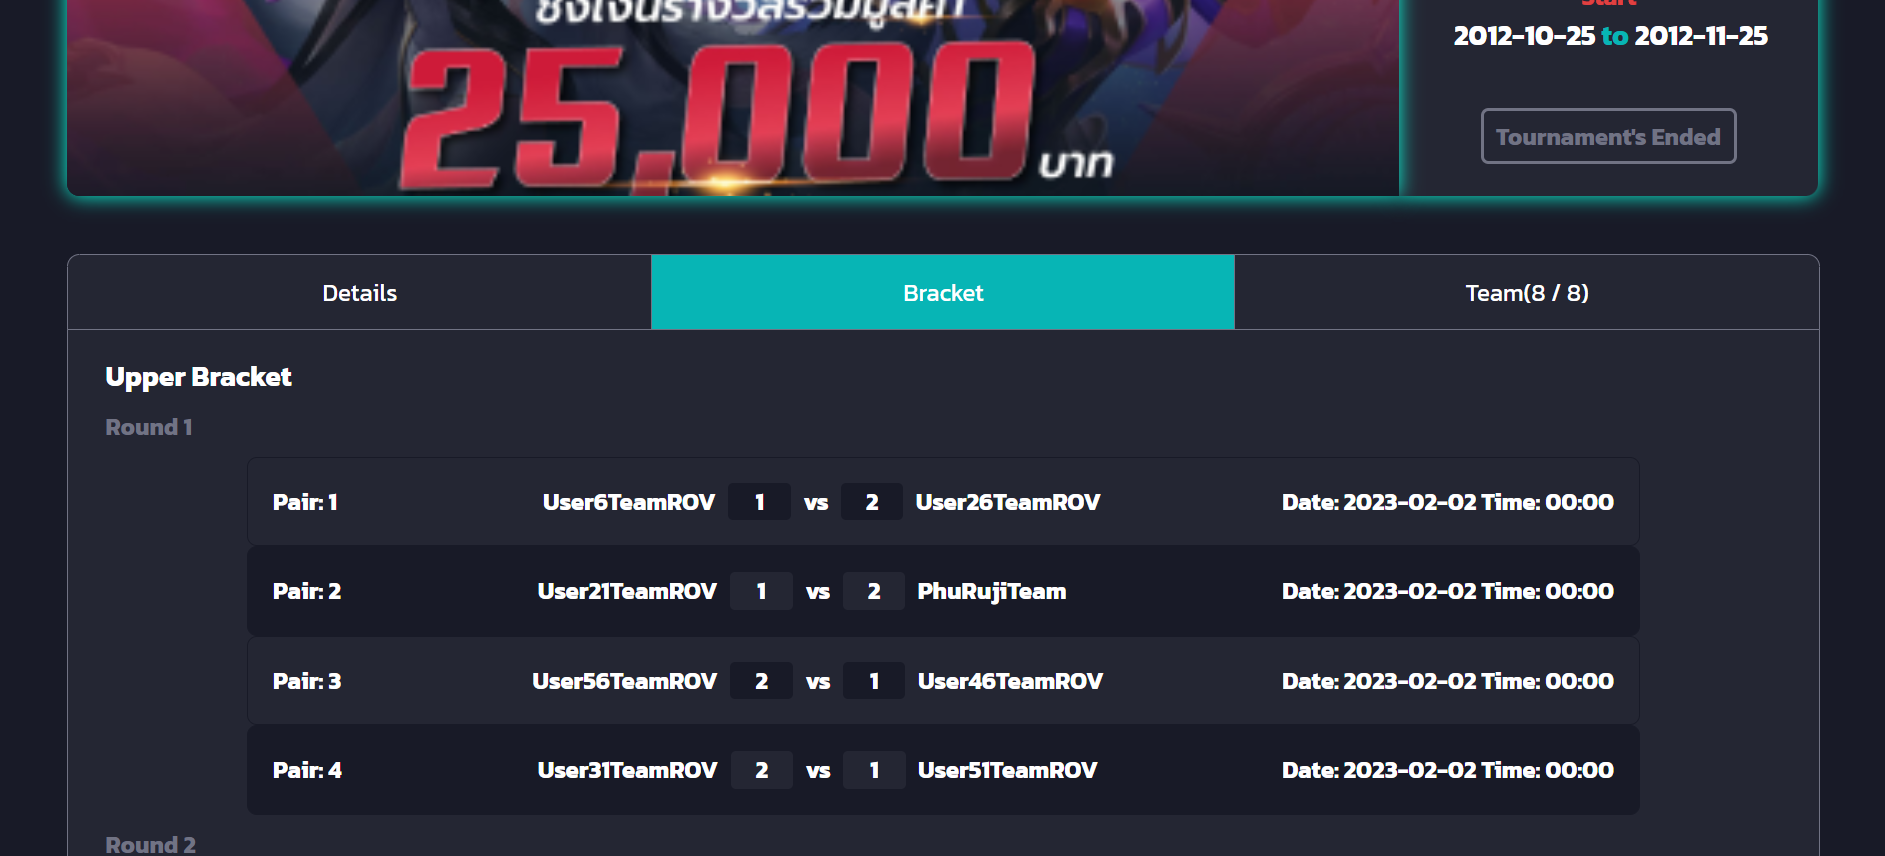
\includegraphics[width=18cm,height=7cm,keepaspectratio]{tournament_each_bracket.png}
      \end{center}
      \caption[หน้ารายละเอียดทัวร์นาเมนต์(ตารางเเข่ง)]{หน้ารายละเอียดทัวร์นาเมนต์(ตารางเเข่ง)}
      \label{fig:หน้ารายละเอียดทัวร์นาเมนต์(ตารางเเข่ง)}
    \end{figure}
    \begin{figure}[ht]
      \begin{center}
      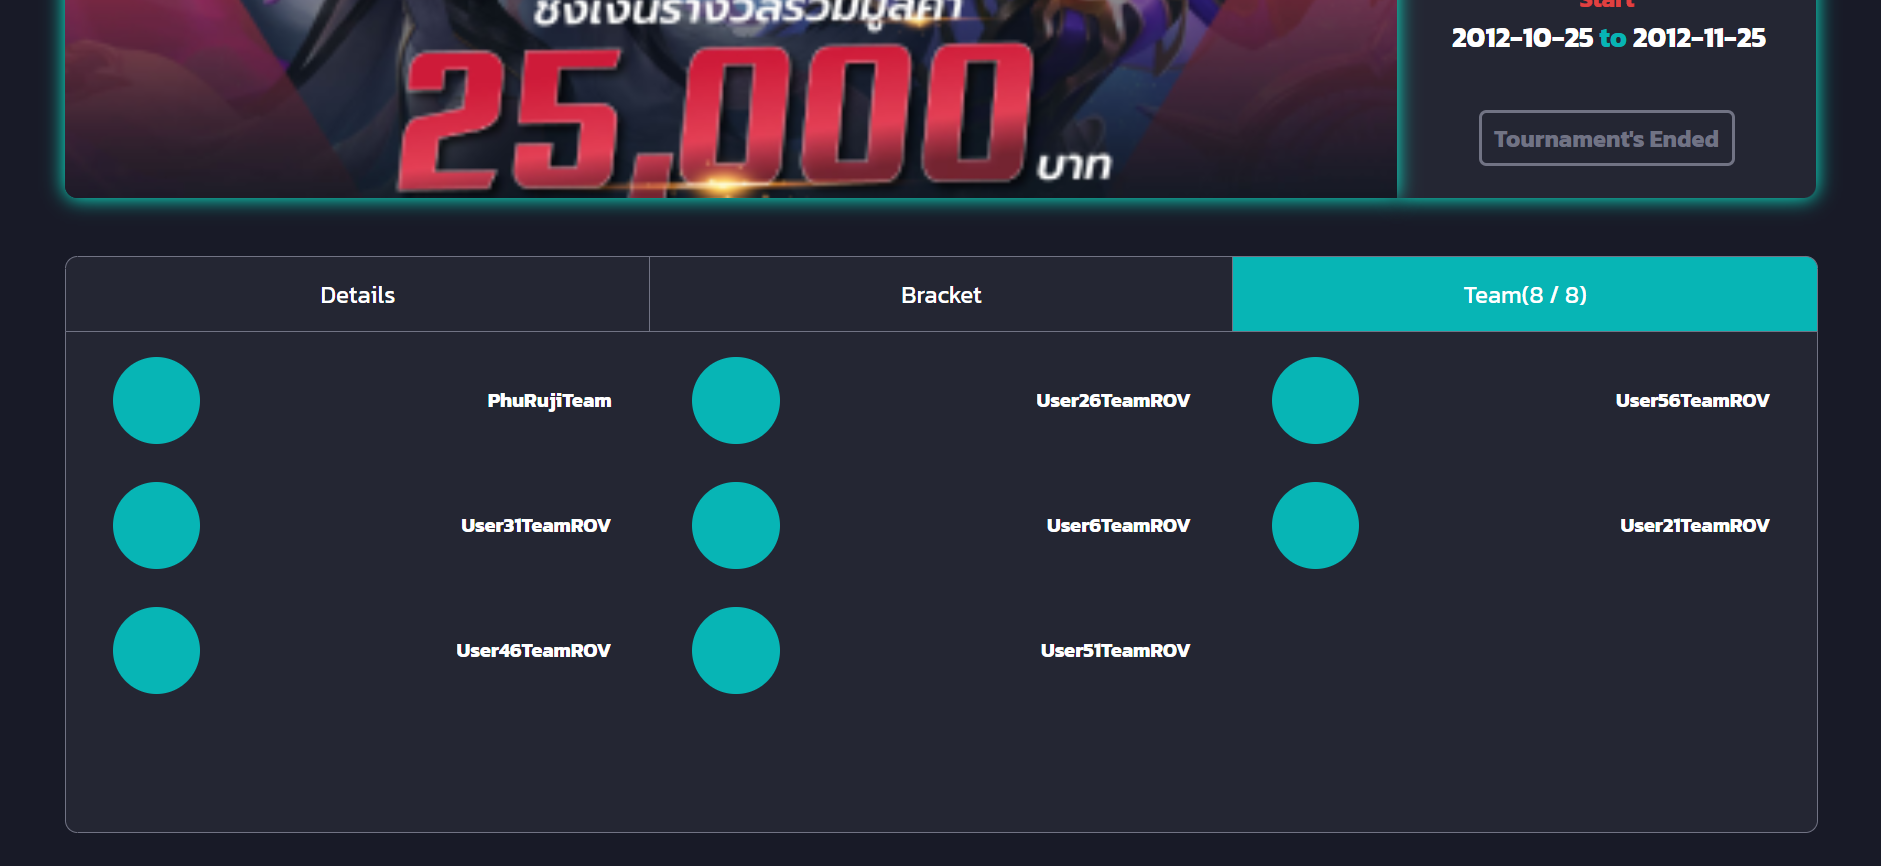
\includegraphics[width=18cm,height=7cm,keepaspectratio]{tournament_each_tj.png}
      \end{center}
      \caption[หน้ารายละเอียดทัวร์นาเมนต์(ทีมที่เข้าร่วม)]{หน้ารายละเอียดทัวร์นาเมนต์(ทีมที่เข้าร่วม)}
      \label{fig:หน้ารายละเอียดทัวร์นาเมนต์(ทีมที่เข้าร่วม)}
    \end{figure}
 
    % create
    \begin{figure}[ht]
      \begin{center}
      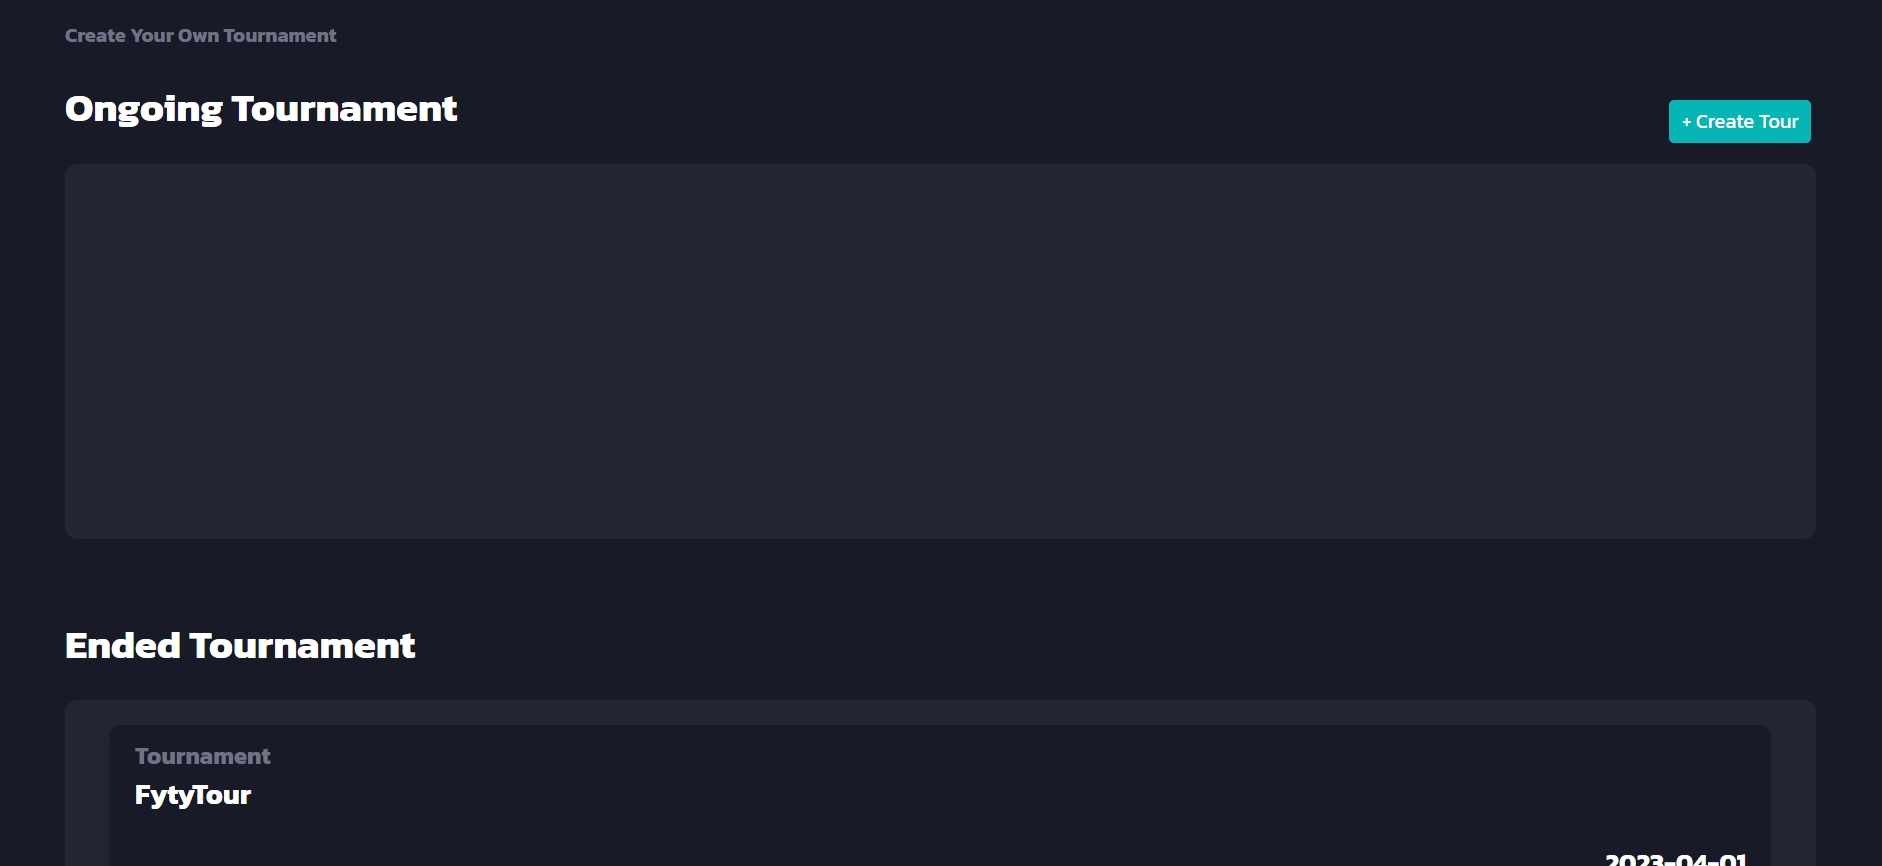
\includegraphics[width=18cm,height=7cm,keepaspectratio]{create_tour.png}
      \end{center}
      \caption[หน้าสร้างทัวร์นาเมนต์]{หน้าสร้างทัวร์นาเมนต์}
      \label{fig:หน้าสร้างทัวร์นาเมนต์}
    \end{figure}
    \begin{figure}[ht]
      \begin{center}
      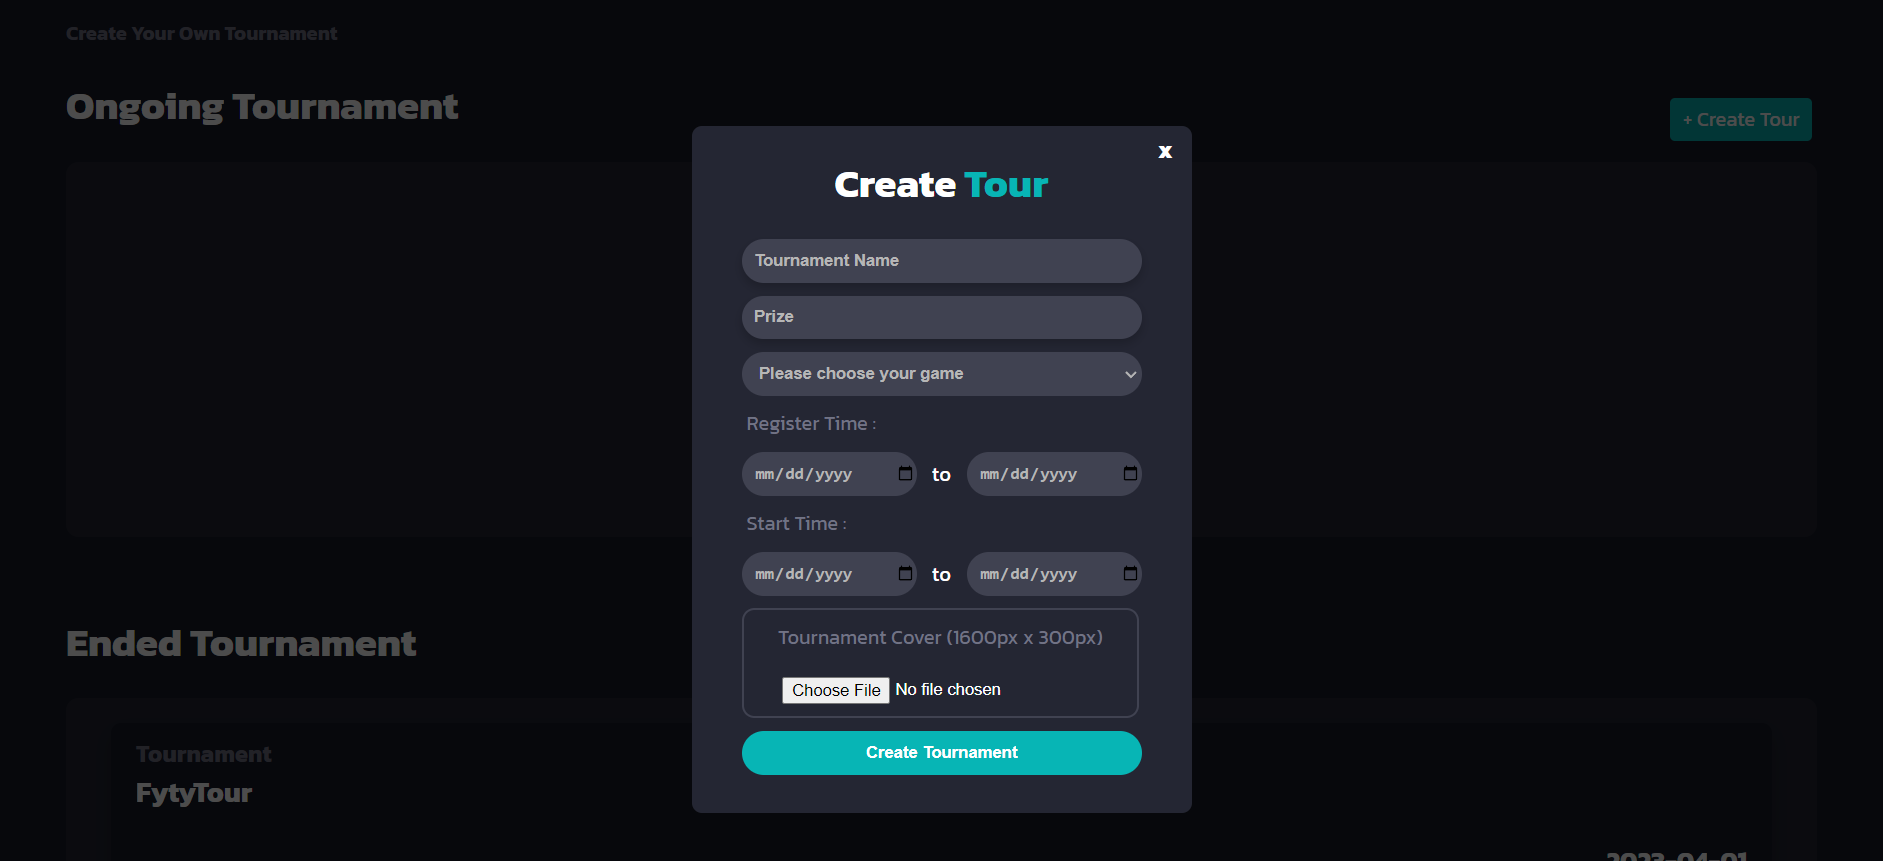
\includegraphics[width=18cm,height=7cm,keepaspectratio]{create_tour_popup.png}
      \end{center}
      \caption[Create Tournament Popup]{Create Tournament Popup}
      \label{fig:Create Tournament Popup}
    \end{figure}

    % profile
    \begin{figure}[ht]
      \begin{center}
      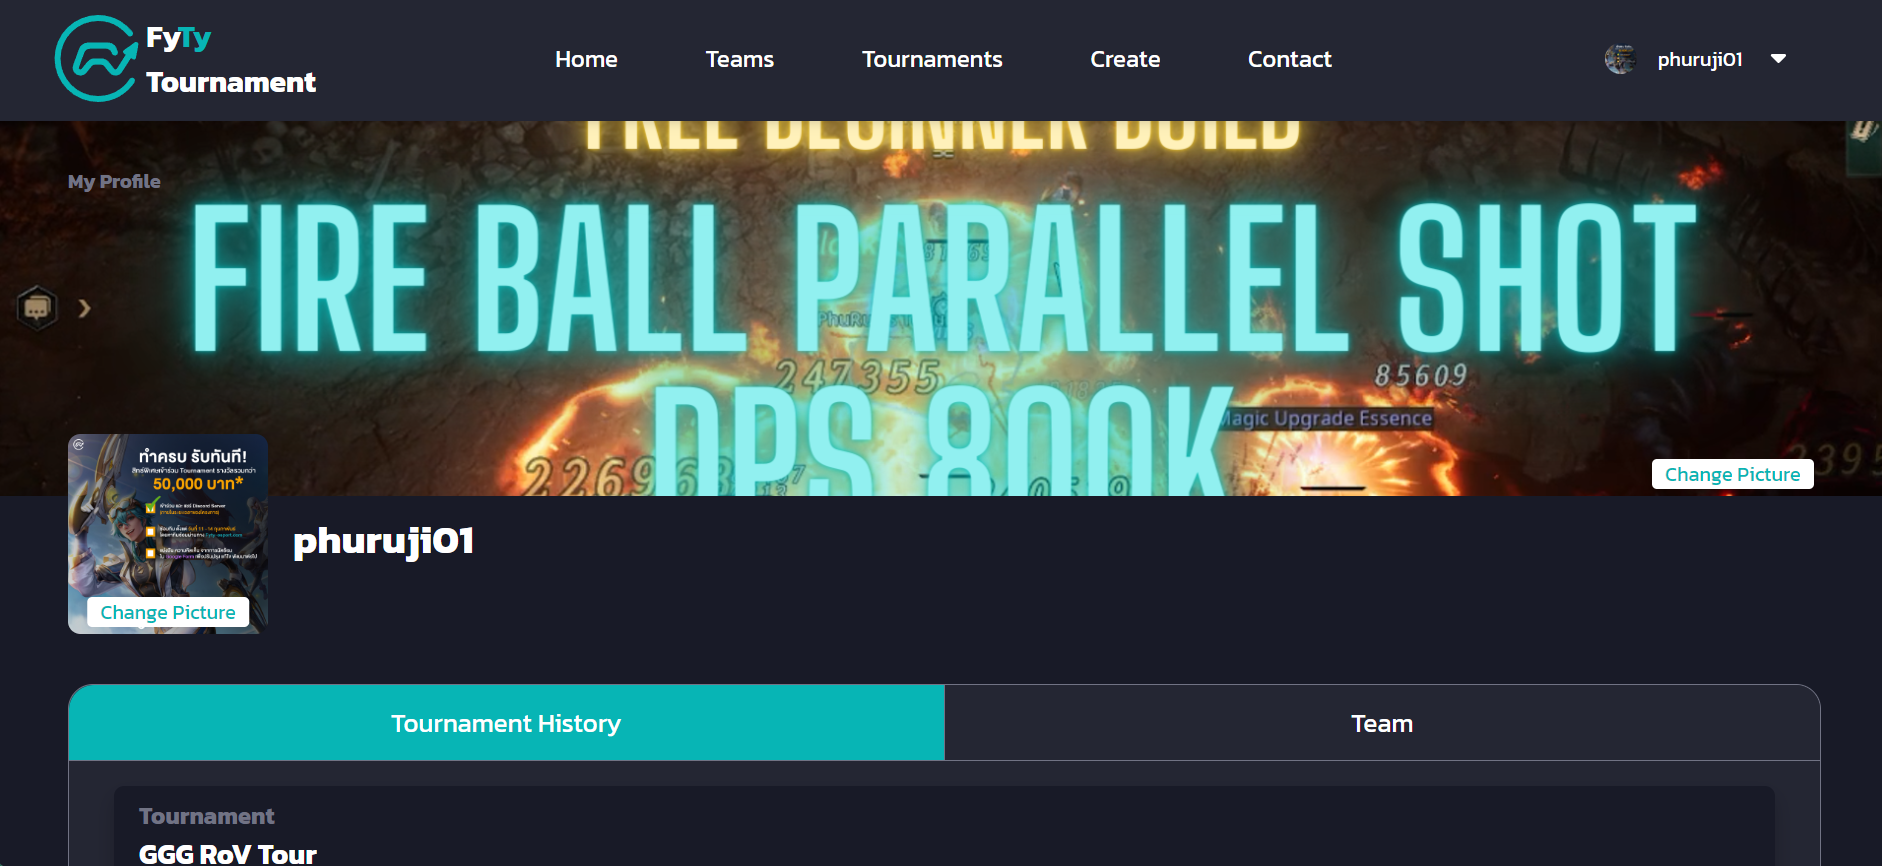
\includegraphics[width=18cm,height=7cm,keepaspectratio]{user_th.png}
      \end{center}
      \caption[หน้ารายละเอียดผู้ใช้(ประวัติการแข่ง)]{หน้ารายละเอียดผู้ใช้(ประวัติการแข่ง)}
      \label{fig:หน้ารายละเอียดผู้ใช้(ประวัติการแข่ง)}
    \end{figure}
    \begin{figure}[ht]
      \begin{center}
      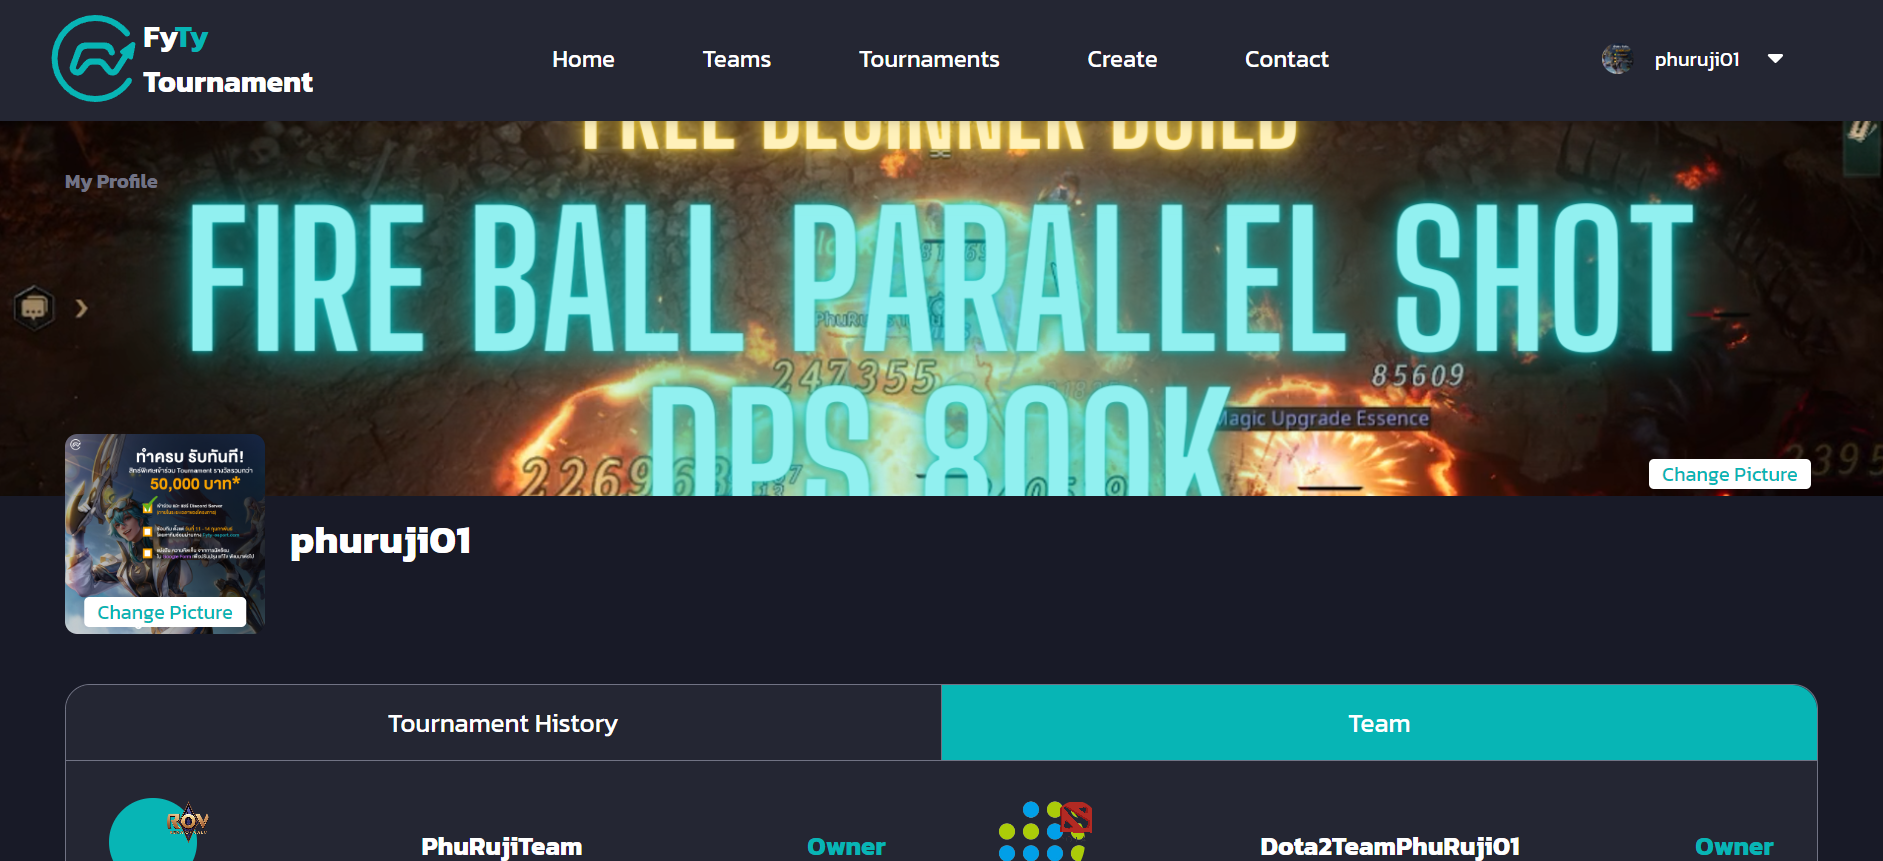
\includegraphics[width=18cm,height=7cm,keepaspectratio]{user_tj.png}
      \end{center}
      \caption[หน้ารายละเอียดผู้ใช้(ทีมที่เคยเข้าร่วม)]{หน้ารายละเอียดผู้ใช้(ทีมที่เคยเข้าร่วม)}
      \label{fig:หน้ารายละเอียดผู้ใช้(ทีมที่เคยเข้าร่วม)}
    \end{figure}

    % schedule
    \begin{figure}[ht]
      \begin{center}
      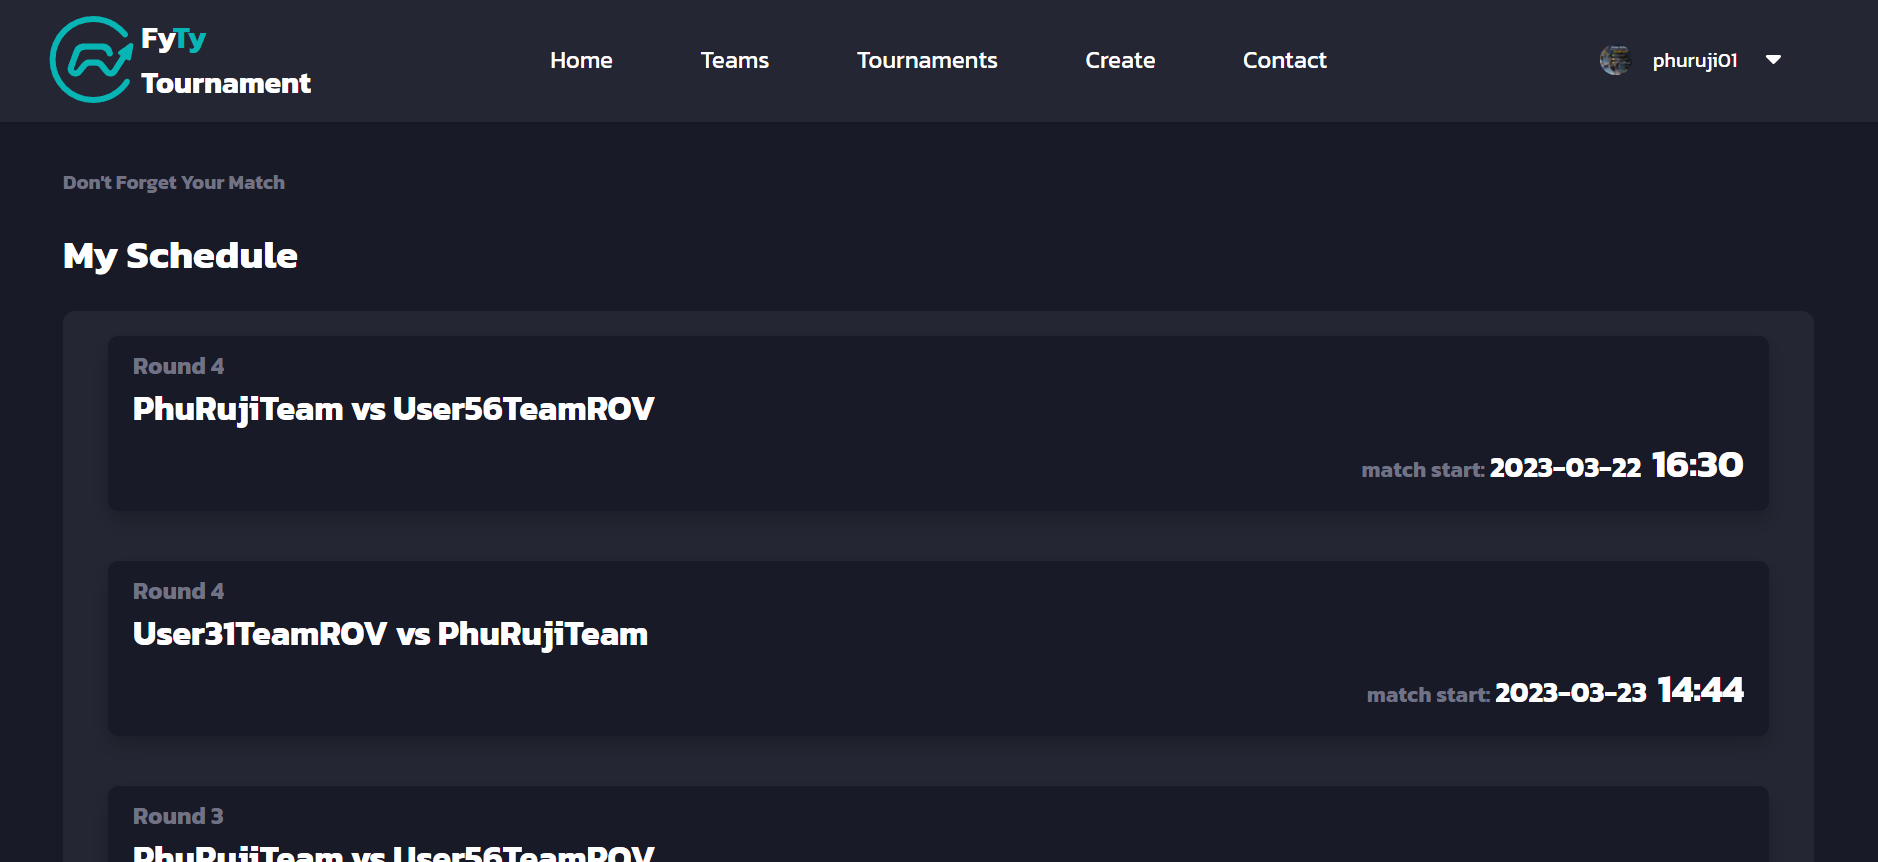
\includegraphics[width=18cm,height=7cm,keepaspectratio]{schedule.png}
      \end{center}
      \caption[ตารางแข่งของเรา]{ตารางแข่งของเรา}
      \label{fig:ตารางแข่งของเรา}
    \end{figure}




\chapter{\ifproject%
\ifenglish Experimentation and Results\else การทดลองและผลลัพธ์\fi
\else%
\ifenglish System Evaluation\else การประเมินระบบ\fi
\fi}

ในบทนี้จะทดสอบเกี่ยวกับการทำงานในฟังก์ชันหลักๆ ของ 2 ฝั่งผู้ใช้งานโดยการให้ทดลองใช้ และทำการสัมภาษณ์

\section{การทดสอบ และผลการทดสอบ ฝั่งผู้เข้าแข่งขัน}
\begin{enumerate}
    \item ทดสอบระบบสร้างทีม - สามารถสร้างทีมได้อย่างรวดเร็วและถูกต้อง
    \item ทดสอบระบบจัดการทีม - สามารถใช้งานได้ง่ายแก้ไขรูปภาพได้ และแสดงรายละเอียดต่างๆของทีมได้ถูกต้อง แต่ยังขาดการจัดการสมาชิกในทีม
    \item ทดสอบระบบจัดการโปรไฟล์ - สามารถใช้งานได้ง่าย และมีข้อมูลรายละเอียดที่จำเป็นครบถ้วน
    \item ทดสอบระบบเลือก และสมัครทัวร์นาเมนต์ - สามารถใช้งานได้ง่าย แต่ต้องใช้เวลาในการอ่านข้อความแจ้งเตือนหากจำนวนสมาชิกทีมไม่ครบเนื่องจากไม่มีการแสดงข้อมูลใดๆที่เกี่ยวกับทีมที่มีในช่องเลือกทีมที่ต้องการเข้า
  \end{enumerate}


\section{การทดสอบ และผลการทดสอบ ฝั่งผู้จัดการแข่งขัน}
\begin{enumerate}
    \item ทดสอบระบบสร้างจัดการทัวร์นาเมนต์ - สามารถสร้างทัวร์นาเมนต์ได้ถูกต้อง แต่อาจมีติดขัดกับการใช้งานเหนื่องจากไม่มีแจ้งเตือนหากใส่ชื่อผิด format ทำให้เหมือนเว็ปค้าง และในเรื่องการจัดการรายละเอียดนั้นสามารถทำได้ง่ายใส่รายละเอียดได้ตามความต้องการ
    \item ทดสอบระบบเดชบอร์ดในการจัดการทัวร์นาเมนต์ - ใช้งานได้ง่ายสะดวกกับการจัดการ
    \item ทดสอบระบบจัดตารางแข่ง - ใช้งานค่อนข้างยากเนื่องจากมีหลายตัวเลือกให้เลือกมากเกินไปทำให้สับสน
  \end{enumerate}


\ifproject
\chapter{\ifenglish Conclusions and Discussions\else บทสรุปและข้อเสนอแนะ\fi}

\section{\ifenglish Conclusions\else สรุปผล\fi}

โครงงานนี้เป็นโครงงานเว็ปแอปพลิเคชั่นที่ใช้ในการจัดการทัวร์นาเมนต์ และเก็บบันทึกสถิติเป็นประวัติผลงาน
ทั้งสำหรับผู้จัดการแข่งขันและผู้เล่นเพื่อนำไปพัฒนาต่อยอดในสายอาชีพนี้ได้ดียิ่งขึ้น
โดยตัวโครงงานนี้สามารถตอบโจทย์การใช้งานได้ในระบบนึงจากการไปให้ผู้ทดสอบที่เป็นคนในสาย E-sport 
ในการทดลองใช้จะติดที่การแสดงผลของตารางแข่ง และนำคนลงสายแข่งที่ยังทำให้บางคนสับสนจากตัวเลือก และเนื้อหาที่แสดงมีจำนวนมากและเฉพาะทาง
\section{\ifenglish Challenges\else ปัญหาที่พบและแนวทางการแก้ไข\fi}

ในการทำโครงงานนี้ พบว่าเกิดปัญหาหลักๆ ดังนี้

\begin{enumerate}
    \item ออกแบบ และวางแผนไม่รัดกุมทั้ง UX/UI และดาต้าเบสทำให้ต้องมีการแก้ไขดาต้าเบส และ UX/UI เฉพาะหน้าเพื่อให้ระบบสามารถทำงานได้อย่างถูกต้อง
    \item เวลาในการพัฒนาโครงงานไม่เพียงพอเนื่องจากมีการเปลี่ยนหัวข้อ และจำนวนคนที่น้อย แนวทางการแก้ไขปัญหา ลดปริมาณของงาน และรายละเอียดที่ไม่จำเป็นลงเพื่อให้ใช้เวลาในการพัฒนาที่น้อยลง 
    เพื่อที่จะได้มีเวลานำเว็ปแอปพลิเคชั่นนี้ไปทำการทดสอบ และเก็บข้อมูล เพื่อที่จะได้ข้อมูลข้อเสนอแนะมาแก้ไข และปรับปรุงให้ดียิ่งขึ้นเหมาะกับกันใช้งานจริงมากยิ่งขึ้น
\end{enumerate}

\section{\ifenglish%
Suggestions and further improvements
\else%
ข้อเสนอแนะและแนวทางการพัฒนาต่อ
\fi
}

ข้อเสนอแนะเพื่อพัฒนาโครงงานนี้ต่อไป มีดังนี้

\begin{enumerate}
    \item ทำตารางแข่งแบบแบบรูปภาพเพื่อให้ดูได้ง่ายและเข้าใจได้ง่าย
    \item ทำระบบแจ้งเตือนเมื่อมีคนขอเข้าทีม หรือใกล้ถึงเวลาแข่ง เพื่อจะได้รับรู้และไม่ลืม โดยหากจะทำระบบนี้ให้รองรับกับการใช้งานจะต้องทำในรูปแบบ Application มือถือเพื่อให้การแจ้งเตือนนั้นมีประสิทธิภาพ
    \item ทำให้หน้าเว็ปไซต์ให้ responsive กับทุกอุปกรณ์ เพื่อการใช้งานได้ในทุกที่ทุกเวลา
\end{enumerate}

\fi

\bibliography{sampleReport}

\ifproject
\normalspacing
\appendix
% ไม่ได้ใช้
\chapter{The first appendix}

Text for the first appendix goes here.

\section{Appendix section}

Text for a section in the first appendix goes here.

test ทดสอบฟอนต์ serif ภาษาไทย

\textsf{test ทดสอบฟอนต์ sans serif ภาษาไทย}

\verb+test ทดสอบฟอนต์ teletype ภาษาไทย+

\texttt{test ทดสอบฟอนต์ teletype ภาษาไทย}

\textbf{ตัวหนา serif ภาษาไทย \textsf{sans serif ภาษาไทย} \texttt{teletype ภาษาไทย}}

\textit{ตัวเอียง serif ภาษาไทย \textsf{sans serif ภาษาไทย} \texttt{teletype ภาษาไทย}}

\textbf{\textit{ตัวหนาเอียง serif ภาษาไทย \textsf{sans serif ภาษาไทย} \texttt{teletype ภาษาไทย}}}

\url{https://www.example.com/test_ทดสอบ_url}

\chapter{\ifenglish Manual\else คู่มือการใช้งานระบบ\fi}

Manual goes here.


%% Display glossary (optional) -- need glossary option.
\ifglossary\glossarypage\fi

%% Display index (optional) -- need idx option.
\ifindex\indexpage\fi

\begin{biosketch}
\begin{center}
  \includegraphics[width=1.5in]{mugshot.jpg}
\end{center}
Your biosketch goes here. Make sure it sits inside
the \texttt{biosketch} environment.
\end{biosketch}
\fi % \ifproject
\end{document}
